\chapter{Vision-Based Multi-Agent Docking with Deep Spiking Neural Networks}

Autonomous docking of multiple agents in close-proximity missions, such as on-orbit servicing, satellite rendezvous, and swarm payload alignment, poses unique challenges in precision, robustness, and energy efficiency. In these missions, a team of robots must cooperate without centralized control, perceive relative pose information under stringent bandwidth and latency constraints, and execute coordinated maneuvers despite dynamic uncertainties and limited onboard resources. To address these challenges, this chapter introduces a fully decentralized, vision-based docking framework for swarm robots, combining \ac{dvs} event streams, \acp{alm}, and a Deep \ac{snn} trained with \ac{stdp}. The sparse, asynchronous output of DVS cameras and the event-driven nature of spiking neural networks contribute to low-latency and energy-efficient control, which supports the development of responsive and resource-aware systems for proximity docking \cite{9138762}.



Prior approaches are often limited by their reliance on centralized coordination, dense frame-based vision pipelines (e.g., frame-based cameras), and rigid control architectures that struggle to scale to multi-agent docking under energy and bandwidth constraints. These limitations hinder their applicability to fully autonomous, decentralized swarm missions in dynamic proximity environments. Building on these insights and addressing the limitations of prior methods, this chapter contributes the following advancements for reliable, efficient, and scalable autonomous docking in multi-agent proximity missions. 

This work presents a biologically interpretable and scalable neuromorphic architecture that achieves end-to-end spiking control for cooperative docking through event-based perception and distributed learning. The main novelties of the proposed system are summarized as follows:

\begin{enumerate}
    \item \textbf{Entropy-based convolution kernel for DVS data:}  
    A new convolution operator is introduced for processing ternary \ac{dvs} events $\{-1,0,+1\}$, where conventional kernels lose information due to polarity sparsity.  
    The proposed variable entropy-based kernel computes spatial importance weights from local event entropy, enabling robust feature extraction from asynchronous visual inputs without frame reconstruction.

    \item \textbf{Short-term memory via bistable neurons:}  
    A population of bistable Izhikevich neurons is designed to emulate a phase–locked–loop–like mechanism in the dynamical sense. Rather than tracking the phase of a sinusoidal input, each neuron possesses an intrinsic oscillatory attractor that becomes entrained by transient DVS events. Once driven into this oscillatory state, the neuron maintains sustained spiking in the absence of further input, analogous to phase capture in a PLL. Event-triggered inhibitory inputs act as a reset mechanism, returning the neuron to its resting equilibrium and effectively unlocking the loop. This bistable excitation–inhibition structure provides short-term temporal memory on the order of tens of milliseconds, preserving recent event activity while guaranteeing temporal continuity in event-driven perception when visual motion ceases.

    \item \textbf{Attention-guided object detection through phase-encoded ALM inhibition:}  
    The first hidden layer includes neurons that emit phase-encoded inhibitory signals synchronized with a physical \ac{alm}. This mechanism uses \ac{alm}s to gate attention toward agents in the \ac{dvs} field of view, suppressing background noise and enhancing agent detection in sparse event streams.

    \item \textbf{Event-triggered policy switching for mission phases:}  
    The second hidden layer incorporates specialized neuron repositories that trigger automatic transitions between mission phases. These transitions are governed by spiking events rather than explicit commands, enabling self-regulated and context-dependent policy switching.

    \item \textbf{Multi-scale synaptic system for visual–motor coordination:}  
    The architecture employs heterogeneous synaptic time constants $(\tau_C, \tau_{\mathrm{STDP}})$ across layers, producing a temporal hierarchy where fast synapses capture rapid \ac{dvs} dynamics and slow synapses stabilize actuator control. This multi-scale structure allows coherent perception–action coupling entirely within the spiking domain.

\end{enumerate}

The remainder of this chapter is organized as follows. The Preliminaries section outlines the docking mission problem with swarm robots, describes the event-based camera simulation setup, details the dynamic models of the payload and agents, and explains the neuron model employed in our network. The Proposed Neuromorphic Framework section presents the architecture of the deep \ac{snn}, including the input layer design with entropy-based adaptive pooling, the encoding configuration, the hidden layers for visual processing and mission phase switching, and the output layer for PWM signal generation. This section also covers the training of the deep \ac{snn} using \ac{stdp}, detailing the reward functions for different hidden layers and the synaptic weight update rules. The Results section evaluates the proposed framework, followed by the Conclusion.


\section{Preliminaries}
\subsection{Problem definition: Docking Missions with Swarm Robots}

Swarm robotics, inspired by the collective behaviors observed in natural systems such as ant colonies, bee swarms, and flocks of birds, represents a promising paradigm for creating intelligent robotic systems capable of performing complex, decentralized tasks. These systems are typically characterized by a number of relatively simple robots that collaborate and coordinate their actions without relying on centralized control. This decentralized approach offers several advantages, including robustness to individual robot failures, flexibility in adapting to changing environments, and scalability to large numbers of agents \cite{dias2021swarm}. 

The desired collective behavior of the swarm emerges from the local interactions among the individual robots and between the robots and their environment. This paradigm contrasts with traditional robotic systems, which often rely on a central controller to dictate the actions of individual robots. The term ``docking missions," in the context of swarm robotics, encompasses a range of cooperative tasks in which multiple robots must achieve a state of connection or close proximity. This includes tasks such as rendezvous, where the objective is for multiple robots to converge at a common location or maintain a defined spatial relationship; assembly, where robots collaboratively work to form a desired structure or connect with other robots or objects to create a larger, functional entity.

In the specific application of this study, the swarm agents are tasked with pushing a payload towards a \ac{scs} to achieve a precise docking alignment. Each agent is equipped with thrusters, allowing them to move in 2D space, and a \ac{dvs} mounted on board provides them with visual feedback about the environment and proximal agents. Additionally, a \ac{dvs} camera is mounted at the center of the \ac{scs}, providing a global event-based view of the payload and agents during docking.

\begin{figure}[H]
    \centering
    \includegraphics[width=1\linewidth]{Figures/3D Environment.pdf}
    \caption{3D schematic of the multi-agent docking mission environment. Multiple agents work collaboratively to push a central payload towards a \ac{scs} for docking alignment.}
    \label{fig:DockingMissionSchematic}
\end{figure}

\begin{figure}[H]
    \centering
    \includegraphics[width=0.9\linewidth]{Figures/Figure 1.pdf}
    \caption{2D representation of robots performing docking mission. Each agent pushes the payload towards the \ac{scs} to align them together. The \ac{scs} and agents are equipped with a \ac{dvs} that streams high-frequency data for the proximity mission.}
    \label{fig:DockingMissionfigure}
\end{figure}


The primary objective of this chapter is to develop a decentralized vision-based swarm docking system utilizing Deep \ac{snn}s trained with \ac{stdp}, which uses the asynchronous, sparse, and high-temporal-resolution output of \ac{dvs} cameras to guide the swarm behavior effectively. Each agent in the swarm runs its own local \ac{snn} onboard, processing sensory information independently and learning control policies in a distributed manner, which allows the swarm to remain scalable and robust to individual agent failures.

In this environment, \ac{alm}s are installed exclusively on the agents to enhance their visibility within the event-based vision system. Each agent only sees its neighboring agents via \ac{dvs} events and does not directly measure their positions. The payload has a considerably larger surface area; as such, it naturally generates sufficient brightness changes to trigger events in the \ac{dvs} sensor without the need for additional illumination. In contrast, the agents are compact and would otherwise produce sparse event activity; thus, their \acp{alm} are used to amplify their visual signatures and ensure reliable detection by the vision system. This configuration simplifies the temporal structure of the event stream while still enabling accurate agent identification and segmentation within the spatiotemporal data.

When the agents are doing rendezvous maneuver and have not made contact with the payload, they rely solely on their onboard \ac{dvs} for environment perception. This allows them to capture events corresponding to nearby agents and the payload. Once an agent makes physical contact with the payload, its onboard force contact sensor activates and the \ac{alm} signal is turned off. The agents' onboard \ac{dvs} data is then replaced by the \ac{scs} \ac{dvs}, providing a more comprehensive and centralized perspective of the payload and the surrounding agents.


\subsection{Event-Based Camera Simulation}

This section presents the simulation methodology for modeling brightness-based visual input and generating asynchronous events for \ac{snn}s using \ac{dvs}. Two distinct \ac{dvs} camera models are used in this study: one mounted on each agent and one placed at a fixed position on the \ac{scs}. Both cameras independently perceive the environment and produce separate event streams based on the change in perceived brightness over time.

The environment is populated by multiple agents and a payload object, each modeled as circular shapes with defined physical properties such as radius and centroid location. Each \ac{dvs} camera discretizes its field of view into a grid of $N_y \times N_x$ pixels, where each pixel corresponds to a fixed location in the simulated physical space. The spatial mapping between the continuous world coordinates and the discrete \ac{dvs} pixel grid is defined through a static transformation.

For each \ac{dvs} view, a brightness map is generated at every simulation time step. Let $X_w$ and $Y_w$ represent the 2D coordinate meshgrids over the \ac{dvs} image plane in world units. The initial brightness grid $E(x,y)$ is set to a constant background value $\zeta_{\text{bg}}$ across all pixels. For each object in the scene, we determine which pixels of the DVS grid fall inside its circular outline. The brightness of these pixels is then calculated using Lambertian reflectance, which varies with the object’s orientation and its distance to each light source.

Let $(x_o, y_o)$ denote the position of an object with radius $r_o$. For each pixel with world coordinates $(x_w, y_w)$, we first compute the squared Euclidean distance to the object center:
\begin{equation}
d^2 = (x_o - x_w)^2 + (y_o - y_w)^2.
\end{equation}

Pixels satisfying $d^2 \leq r_o^2$ are considered to lie within the object’s projection. For these pixels, brightness is calculated based on Lambertian reflectance with multiple light sources. Let $(x^{(l)}_s, y^{(l)}_s)$ denote the position of the $l$-th light source. We define the vector from the pixel to the light source as:
\begin{equation}
\mathbf{L}_{\text{light}}^{(l)} = 
\begin{bmatrix}
x_w - x^{(l)}_s \\
y_w - y^{(l)}_s
\end{bmatrix}, \qquad
||\mathbf{L}_{\text{light}}^{(l)}|| = \sqrt{(x_w - x^{(l)}_s)^2 + (y_w - y^{(l)}_s)^2},
\end{equation}
similarly, the vector from the pixel to the object center is:
\begin{equation}
\mathbf{L}_{\text{center}} = 
\begin{bmatrix}
x_o - x_w \\
y_o - y_w
\end{bmatrix}, \qquad
||\mathbf{L}_{\text{center}}|| = \sqrt{(x_o - x_w)^2 + (y_o - y_w)^2}.
\end{equation}

The angle $\psi^{(l)}$ between these two vectors is used to compute the cosine-based brightness contribution from light source $l$:
\begin{equation}
\psi^{(l)} = \arccos\left(\frac{\mathbf{L}_{\text{light}}^{(l)} \cdot \mathbf{L}_{\text{center}}}{||\mathbf{L}_{\text{light}}^{(l)}|| \cdot ||\mathbf{L}_{\text{center}}|| + \varepsilon}\right),
\end{equation}
\begin{equation}
\zeta^{(l)} = \max\left(0, \cos(\psi^{(l)}) \cdot 0.5 + 0.5\right),
\end{equation}
where $\varepsilon$ is a small constant to avoid division by zero. The final brightness value at each pixel is computed as the maximum contribution across all light sources and overlapping objects:
\begin{equation}
E(x_w, y_w) = \max\left( \zeta_{\text{bg}}, \max_{\text{objects}} \max_l \zeta^{(l)} \right).
\end{equation}

Once the brightness map $E(x,y)$ is generated, it is passed to the event generation module that models the behavior of the \ac{dvs} sensor. To emulate the logarithmic response of biological photoreceptors, the brightness is first clamped from below to a minimum threshold $\zeta_{\min}$ (i.e., any value below $\zeta_{\min}$ is raised to $\zeta_{\min}$) and transformed into logarithmic intensity \cite{9138762}:
\begin{equation}
E_{\text{clamped}}(x,y) = \max(E(x,y), \zeta_{\min}), 
\end{equation}
\begin{equation}
\mathcal{L}_{\text{current}}(x,y) = \ln(E_{\text{clamped}}(x,y)).
\end{equation}

The temporal contrast is computed as the difference between the current and previously stored logarithmic intensity and integrated into a membrane potential variable $U(x,y)$ for each pixel \cite{graca2025towards}:
\begin{equation}
\Delta \mathcal{L}(x,y) = \mathcal{L}_{\text{current}}(x,y) - \mathcal{L}_{\text{prev}}(x,y),
\end{equation}
\begin{equation}
U_t(x,y) = U_{t-1}(x,y) + \Delta \mathcal{L}(x,y).
\end{equation}

The membrane potential is bounded from below at $-\vartheta_{\text{on}}$ to prevent excessive accumulation of tiny negative values in dark regions, thereby improving numerical stability. In practice, a real \ac{dvs} stops integrating once intensity becomes constant, but in simulation, small numerical biases can accumulate over time. To prevent this artificial drift from repeatedly triggering OFF events in static dark regions, we bound the potential to a lower limit instead of allowing it to integrate indefinitely.

The \ac{dvs} event generation rule triggers ON and OFF events based on threshold crossing behavior. Define thresholds $\vartheta_{\text{on}} > 0$ and $\vartheta_{\text{off}} > 0$. For each pixel, if:
\begin{equation}
\left\{
\begin{aligned}
&\text{if } U(x,y) \geq \vartheta_{\text{on}}: 
&& e(x,y) = +1, 
&& U(x,y) \leftarrow U(x,y) - \vartheta_{\text{on}}, \\
&\text{if } U(x,y) \leq -\vartheta_{\text{off}}: 
&& e(x,y) = -1, 
&& U(x,y) \leftarrow U(x,y) + \vartheta_{\text{off}}.
\end{aligned}
\right.
\end{equation}

Otherwise, no event is generated and $e(x,y) = 0$. These updates are performed for both agent-mounted and \ac{scs}-mounted \ac{dvs} views independently, using their respective brightness maps and potential histories. The $\mathcal{L}_{\text{current}}$ map is stored as $\mathcal{L}_{\text{prev}}$ for the next time step. This detailed simulation allows each agent to perceive a localized view of the environment while the \ac{scs} maintains a global perspective. 


% Read these papers:
% \begin{itemize}
%     \item Autonomous in-orbit satellite assembly from a modular heterogeneous swarm
%     \item Robust event-triggered game-based attitude control for on-orbit assembly
%     \item Centralized visual-based navigation and control of a swarm of satellites for on-orbit servicing
%     \item Federated Multi-Agent Mapping for Planetary Exploration
% \end{itemize}


\subsection{Dynamic Model of the Payload and Agents} 
\label{sec:agent_dynamics}

Each agent in the swarm is modeled as a point mass of mass \( m \) and radius \(R\). The dynamic state of each agent includes its position, velocity, thrust-based control forces, and interaction forces arising from \emph{agent--agent} collisions. A central payload object with its own dynamics is influenced by contacts with the agents via a time-limited attachment rule (described below).

The state of agent \( i \) at time \( t \) is defined as $\mathbf{p}_i(t) = \begin{bmatrix} X_i(t) \\ Y_i(t) \end{bmatrix}$ and $\mathbf{V}_i(t) = \begin{bmatrix} V_{x_i}(t) \\ V_{y_i}(t) \end{bmatrix}$, and the control thrusts along the X and Y axes are derived from spike activity in the output layer of a \ac{snn}. Agent--agent interactions are modeled using a spring–damper system. Let agent \( a \) with position \( \mathbf{p}_a \), velocity \( \mathbf{V}_a \), and radius \( R_a \) interact with agent \( b \) with position \( \mathbf{p}_b \), velocity \( \mathbf{V}_b \), and radius \( R_b \). The collision force is
\begin{align}
    \Delta_{ab} &= R_a + R_b - \|\mathbf{p}_a - \mathbf{p}_b\|, \\
    \mathbf{n}_{ab} &= \frac{\mathbf{p}_a - \mathbf{p}_b}{\|\mathbf{p}_a - \mathbf{p}_b\|}, \\
    \mathbf{V}_{ab}^{\mathrm{rel}} &= \mathbf{V}_a - \mathbf{V}_b, \\
    \mathbf{F}_{ab}^{\text{coll}} &= k \,\Delta_{ab}\,\mathbf{n}_{ab}
    \;+\; c \,\max\!\bigl(-(\mathbf{V}_{ab}^{\mathrm{rel}}\!\cdot\!\mathbf{n}_{ab}),\,0\bigr)\,\mathbf{n}_{ab},
\end{align}
\noindent where \( k \) is the stiffness and \( c = 2\zeta\sqrt{k\,m_{\mathrm{eff}}} \) is a near-critically damped coefficient with reduced mass \( m_{\mathrm{eff}} = \frac{m_a m_b}{m_a + m_b} \) (damping acts only on approach). The force on \( a \) is \( \mathbf{F}_{ab}^{\text{coll}} \) and on \( b \) is \( -\mathbf{F}_{ab}^{\text{coll}} \).

The total force on a free agent \( a \) is the sum of its thrust and agent–agent collisions:
\begin{equation}
    \mathbf{F}_a^{\text{total}}(t) = \mathbf{F}_a^{\text{thrust}}(t) + \sum_{b \neq a} \mathbf{F}_{ab}^{\text{coll}}(t),
\end{equation}
\noindent and its motion follows Newton’s second law
\begin{equation}
    \frac{d^2 \mathbf{p}_a(t)}{dt^2} = \frac{\mathbf{F}_a^{\text{total}}(t)}{m_a}.
\end{equation}

Agent–payload interactions are not modeled via a spring–damper system; instead, first contact triggers a rigid attachment for a fixed duration \( \tau_{\text{attach}}=10\,\mathrm{s} \). Let \( \mathbf{p}_P, \mathbf{V}_P, R_P, m_P \) be the payload pose, velocity, radius, and mass. Attachment is triggered when
\begin{equation}
    \Delta_{iP}(t) \;=\; R_i + R_P - \|\mathbf{p}_i(t) - \mathbf{p}_P(t)\| \;>\; 0.
\end{equation}
While attached, the agent’s pose is locked to a fixed offset \( \boldsymbol{\delta}_i \) on the payload surface and shares its velocity:
\begin{equation}
    \mathbf{p}_i(t) = \mathbf{p}_P(t) + \boldsymbol{\delta}_i,\qquad
    \mathbf{V}_i(t) = \mathbf{V}_P(t), \qquad t\in[t_0,\, t_0+\tau_{\text{attach}}].
\end{equation}
During attachment, the agent’s thrust is routed to the payload, and the payload integrates with the \emph{effective mass} of itself plus all currently attached agents:
\begin{align}
    \mathcal{Z}(t) &:= \{\,i \;|\; i \text{ attached at } t \,\}, \\
    m_{\mathrm{eff}}(t) &= m_P + \sum_{i\in\mathcal{Z}(t)} m_i, \\
    \mathbf{F}_P^{\text{total}}(t) &= \sum_{i\in\mathcal{Z}(t)} \mathbf{F}_i^{\text{thrust}}(t), \\
    \frac{d^2 \mathbf{p}_P(t)}{dt^2} &= \frac{\mathbf{F}_P^{\text{total}}(t)}{m_{\mathrm{eff}}(t)}.
\end{align}
After \( \tau_{\text{attach}} \), the agent detaches and resumes free-agent dynamics.

These equations describe the continuous-time dynamics of the agents and the payload with agent–agent collision handling, attachment-mediated agent–payload coupling, thrust routing to the payload during attachment, and mass aggregation for the translational motion of the combined system (center-of-mass dynamics) over the attachment interval. Rotational dynamics of the payload are neglected in this simplified model.

% \paragraph{Velocity feedback and speed governor.}
% When an agent has inertia, an action change does not instantaneously reverse motion. If the \ac{snn} correctly commands a turn but the velocity has not yet changed sign, reward terms based on instantaneous motion direction can remain negative during the transient, producing misleading feedback. To avoid pushing the agent into a regime where the available thrust cannot promptly reverse the motion, we add a velocity feedback loop that limits speed.

% Let $\mathbf{u}_{\text{snn}}(t)\in\mathbb{R}^2$ be the thrust command decoded from the output layer
% (positive direction is $+\!X,+\!Y$), and $\|\mathbf{u}_{\text{snn}}(t)\|\le F_{\max}$.
% The translational dynamics for a free agent of mass $m$ are
% \begin{equation}
% \dot{\mathbf{p}}(t) = \mathbf{v}(t),\qquad
% m\,\dot{\mathbf{v}}(t) = \mathbf{u}_{\text{tot}}(t) + \mathbf{f}_{\text{coll}}(t),
% \end{equation}
% where $\mathbf{f}_{\text{coll}}$ is the spring–damper collision force defined above and
% $\mathbf{u}_{\text{tot}}$ is the thrust after speed regulation.

% We define a smooth, axis–wise braking term that activates only when the speed magnitude exceeds a cap $V_{\max}>0$:
% \begin{align}
% \sigma(v;V_{\max},\delta) &= \tfrac{1}{2}\!\left(1+\tanh\!\frac{|v|-V_{\max}}{\delta}\right)\in[0,1],\\
% u_{\text{gov},x} &= -\,m\,K_g\,\sigma(v_x;V_{\max},\delta)\,v_x,\qquad
% u_{\text{gov},y} = -\,m\,K_g\,\sigma(v_y;V_{\max},\delta)\,v_y,
% \end{align}
% with $K_g>0$ a governor gain and $\delta>0$ a small smoothing band.
% The total commanded thrust (per axis) is the sum of the \ac{snn} command and the governor, saturated at the hardware limit:
% \begin{equation}
% \mathbf{u}_{\text{tot}} \;=\;
% \operatorname{sat}_{F_{\max}}\!\bigl(\,\mathbf{u}_{\text{snn}} + \mathbf{u}_{\text{gov}}\,\bigr),
% \qquad
% \operatorname{sat}_{F_{\max}}(\mathbf{w})
% = \bigl(\max\!\bigl(\!-F_{\max}, \min\!(w_x,F_{\max})\bigr),\;
%           \max\!\bigl(\!-F_{\max}, \min\!(w_y,F_{\max})\bigr)\bigr).
% \end{equation}

% This governor behaves as a viscous brake that is \emph{off} when $|v_x|,|v_y|\le V_{\max}$ and smoothly
% increases beyond that range, ensuring the agent remains in a controllable speed envelope where a change of thrust can reverse its motion within a short transient.
% Practically, this reduces reward ambiguity during reversals: although the \ac{snn} may select the correct opposite action, the velocity direction—and thus direction-based reward—lags until inertia is overcome. The governor limits the peak speed so that reversals occur quickly, aligning reward with intent and stabilising learning.

% During rigid attachment to the payload, the agent’s thrust is routed to the payload and the same form of dynamics applies to the payload with the aggregated effective mass.

The agent actuation in the simulation follows a thruster model, in which each nozzle exhibits a \ac{mib} of 50 ms \cite{botelho2024explicit}. A \ac{mib} is the thruster's minimum non‑zero on‑time (i.e., the smallest pulse duration the thruster can produce). Consequently, thrust updates are issued at a fixed actuation interval $T_{\mathrm{mib}}=50\ \mathrm{ms}$, while the physics are integrated with a smaller step $\Delta t>0$. Let $k\in\mathbb{N}$ index the \ac{mib} windows and define $t\in[kT_{\mathrm{mib}},(k{+}1)T_{\mathrm{mib}})$. The thrust decoded from the output layer of the \ac{snn}, $\mathbf{u}_{\mathrm{snn}}(t)\in\mathbb{R}^2$, is zero–order–held over each window and quantized by the thruster on–time constraint:
\begin{equation}
\mathbf{u}_{\mathrm{thr}}(t)
\,=\,F_{\max}\,\mathbf{s}_k,\qquad
\mathbf{s}_k\in\{-1,0,+1\}^2\ \text{(X- and Y-components)},\qquad
 t\in[kT_{\mathrm{mib}},(k{+}1)T_{\mathrm{mib}}),
\label{eq:MIB-thrust}
\end{equation}
where the sign vector $\mathbf{s}_k$ is inferred from the spike counts in the last decision window. For example,
\begin{equation*}
s_{k,x}=\operatorname{sign}\big(N_{x^-}(k)-N_{x^+}(k)\big),\qquad
s_{k,y}=\operatorname{sign}\big(N_{y^-}(k)-N_{y^+}(k)\big),\qquad \operatorname{sign}(0)=0.
\end{equation*}
Here $N_{x^-}(k)$ and $N_{x^+}(k)$ denote the spike counts of the output neurons encoding the negative and positive $X$ thrust directions, respectively, during \ac{mib} window $k$ (and analogously $N_{y^-},N_{y^+}$ for the $Y$ axis). The translational dynamics of a free agent of mass $m$ are
\begin{equation}
\dot{\mathbf{p}}(t)=\mathbf{V}(t),\qquad
m\,\dot{\mathbf{V}}(t)=\mathbf{u}_{\mathrm{thr}}(t)+\mathbf{f}_{\mathrm{coll}}(t),
\end{equation}
where $\mathbf{f}_{\mathrm{coll}}(t)$ denotes the spring–damper collision force modeled previously. 
The thruster \ac{mib} fixes the pulse width. As a result, the thrust command is applied in discrete time intervals, while the system dynamics remain continuous. Whenever $\mathbf{s}_k \neq \mathbf{0}$, a constant thrust of magnitude $F_{\max}$ is held over the entire interval $[kT_{\mathrm{mib}}, (k{+}1)T_{\mathrm{mib}})$. Within that interval, no change in thrust direction or magnitude is possible.

% Because the pulse–width is fixed by the MIB, the actuation becomes hybrid and time–quantized: whenever $\mathbf{s}_k\neq\mathbf{0}$ the commanded magnitude $F_{\max}$ is maintained for the entire interval $[kT_{\mathrm{mib}},(k{+}1)T_{\mathrm{mib}})$, precluding mid–window reversals.

% To keep the agent within a controllable speed envelope under the discrete thrust actuation, a velocity governor is applied synchronously with the \ac{snn} output at every interval $T_{\mathrm{mib}}$.  
% At each update step $k$, the instantaneous velocity $\mathbf{V}_k=[V_{x,k},V_{y,k}]^{\mathsf{T}}$ is compared against a predefined speed limit $V_{\max}>0$.  
% When the absolute velocity in an axis exceeds this limit, a corrective force proportional to the excess speed is generated; otherwise, the governor remains inactive.  
% The per–axis control law is expressed as
% \begin{equation}
%     u_{\mathrm{gov},x}[k] = -\,m\,K_g\,\big(|V_{x,k}|-V_{\max}\big)_{+}\,\operatorname{sign}(v_{x,k})
% \end{equation}
% \begin{equation}
%     u_{\mathrm{gov},y}[k] = -\,m\,K_g\,\big(|V_{y,k}|-V_{\max}\big)_{+}\,\operatorname{sign}(v_{y,k})
% \end{equation}
% where $(x)_{+}=\max(0,x)$ denotes the positive–part operator, returning $x$ if $x>0$ and $0$ otherwise, and $K_g>0$ is the feedback gain. Because the governor is evaluated at the same discrete interval as the \ac{snn} output, its effect appears as an intermittent corrective pulse rather than a continuous viscous drag. It effectively prevents the agent from exceeding the controllable velocity envelope, ensuring that thrust reversals can occur within a few actuation periods despite the inertia and the 50\,ms minimum–impulse constraint. This interaction between discrete actuation and velocity feedback introduces nonconvexity into optimization–based controllers such as Model-Predictive Contoller \cite{mei2025modeling}, since the control inputs $\mathbf{s}_k\in\{-1,0,+1\}^2$ and their timing are inherently discrete and coupled to the system dynamics. In contrast, the proposed \ac{snn} adapts to this hybrid behavior by learning spike patterns that anticipate the motor’s quantized response, thereby compensating for the nonlinear and discontinuous actuation without requiring explicit mixed–integer optimization.

\subsection{Neuron model}

Biologically inspired spiking neuron models often exhibit rich dynamical behaviors such as excitability, bursting, and bistability. The well-known Izhikevich model \cite{izhikevich2003simple} strikes a balance between biophysical realism and computational efficiency, using only two ordinary differential equations plus a reset condition. The standard Izhikevich model is given by
\begin{equation}
\begin{cases}
\displaystyle \frac{dv}{dt} \;=\; 0.04\,v^2 \;+\; 5\,v \;+\; 140 \;-\; u \;+\; I(t), \\[6pt]
\displaystyle \frac{du}{dt} \;=\; a\,\bigl(b\,v \;-\; u\bigr),
\end{cases}
\label{eq:izhikevich}
\end{equation}
with a reset rule:
\begin{equation}
\text{if } v \ge 30\text{ mV, then }
\begin{cases}
v \leftarrow c,\\
u \leftarrow u + d.
\end{cases}
\end{equation}

\noindent where $a$ and $\mathbf{B}$ are the neuron parameters, $v$ is the membrane potential (in mV), $u$ is a slow recovery variable, $I(t)$ is the external input current, and $c$ and $d$ define how the system is reset after a spike.

% \subsection{Random Synaptic Weight Initialization}

% The initial synaptic weight matrix \(\mathbf{W}\in\mathbb R^{N_\mathrm{post}\times N_\mathrm{pre}}\) is created based on the binary connectivity matrix \(\mathcal C\in\{0,1\}^{N_\mathrm{post}\times N_\mathrm{pre}}\), where \(N_\mathrm{post}\) denotes the number of postsynaptic neurons and \(N_\mathrm{pre}\) denotes the number of presynaptic neurons. Each element of \(\mathbf{W}\) is given by


% \begin{equation}
% \mathbf{W}(i,j)=
% \begin{cases}
% w_{ij}, & \mathcal C(i,j)=1,\\
% 0,       & \text{otherwise,}
% \end{cases}
% \end{equation}
% so that non‐existent connections remain zero.

% A scalar parameter \(p_{\mathrm{active}}\in(0,1]\) (default value \(0.10\)) sets the fraction of the total incoming synaptic strength that may be simultaneously active for each neuron. If \(\mathcal{W}_{\mathrm{in}}\) denotes the maximum allowable total input strength for a given postsynaptic neuron, then the threshold \(\Theta \;=\;\frac{\mathcal{W}_{\mathrm{in}}}{p_{\mathrm{active}}}\) defines the upper bound on the raw sum of incoming weights before normalization. In other words, if the sum of a neuron’s initial synaptic weights exceeds \(\Theta\), the weights are rescaled so that the effective input does not surpass the prescribed maximum.

% The algorithm proceeds layer by layer. For layer index \(\ell=2,\dots,n_{\mathrm{L}}\), let \(\mathcal P_\ell\) be the set of postsynaptic neuron indices in layer \(\ell\) and \(\mathcal Q_{\ell-1}\) the set of presynaptic indices in the previous layer. To generate a spatially smooth random gradient over the presynaptic population, the \(N=|\mathcal Q_{\ell-1}|\) presynaptic indices are embedded onto a two‐dimensional grid. For simplicity, we assume that the presynaptic neurons can be arranged on a 2D grid arrangement of neurons of size \(\sqrt{N}\times \sqrt{N}\), so that each neuron is assigned integer coordinates,
% \begin{equation}
% \{(x_k,y_k)\}_{k=1}^N \;\subset\; \{1,\dots,\sqrt{N}\}\times\{1,\dots,\sqrt{N}\},
% \end{equation}
% and a random center
% \begin{equation}
% \boldsymbol{\mathcal{O}}
% =\Bigl(\tfrac{\sqrt N+1}2,\tfrac{\sqrt N+1}2\Bigr)
% +\varepsilon,\quad
% \varepsilon\sim\mathcal U\!\bigl([-0.5\sqrt N,\,0.5\sqrt N]^2\bigr),
% \end{equation}
% where, \(\varepsilon\) is sampled from a uniform distribution and width \(\sigma=\sqrt N/3\) define a Gaussian kernel with additive uniform noise:
% \begin{equation}
% g_k
% =\exp\!\Bigl(-\tfrac{(x_k-\mu_x)^2+(y_k-\mu_y)^2}{2\sigma^2}\Bigr)
% +\eta_k,\quad
% \eta_k\sim\mathcal U([-0.5,\,0.5]).
% \end{equation}
% normalizing \(g_k\) by its maximum,
% \begin{equation}
% \overline{g}_k
% =\frac{g_k}{\max \{g_k\}},
% \end{equation}
% yields values in \([0,1]\). These are then mapped into the allowed weight range by
% \begin{equation}
% w_k
% = I_{\min} + (I_{\max}-I_{\min})\,\overline{g}_k.
% \end{equation}

% For each postsynaptic neuron \(i\in\mathcal P_\ell\), let \(\mathcal I_i\subset\{1,\dots,N\}\) denote the indices of those presynaptic neurons whose positions on the 2D grid correspond to nonzero connections. The raw incoming weights for neuron \(i\) are then \(\{w_j\}_{j\in\mathcal I_i}\). If their sum exceeds the threshold \(\Theta\), they are uniformly rescaled:
% \begin{equation}
% \text{if }\sum_{j\in\mathcal I_i}w_j>\Theta,\quad
% w_j\;\leftarrow\;
% w_j\,\frac{\Theta}{\sum_{k\in\mathcal I_i}w_k},
% \quad j\in\mathcal I_i.
% \end{equation}

% Finally, these weights are placed into the initialization matrix by
% \begin{equation}
% \mathbf{W}\bigl(i,\mathcal Q_{\ell-1}[j]\bigr)
% = w_j,
% \quad j\in\mathcal I_i,
% \end{equation}
% ensuring that each neuron’s incoming synaptic strengths obey both the spatial gradient structure and the total input constraint.

% \subsection{Analytic determination of inhibitory synaptic weight (Bistability neuron)}
% We consider the Izhikevich ``Bistability'' neuron with parameters \(a=1,\; b=1.5,\; c=-60,\; d=0\) receiving an excitatory drive \(I_{\rm exc}(t)\) and a fixed inhibitory pulse \(I_{\rm inh}(t)\) \cite{izhikevich2004model}. Spiking ceases when the \(v\)-nullcline in~\eqref{eq:izhikevich}
% \begin{equation}
% 0.04\,v^2 + 5v + 140 - u + I = 0
% \end{equation}
% touches its extremum, i.e.,
% \begin{equation}
% \frac{\partial}{\partial v}\bigl(0.04\,v^2 + 5v + 140 - u + I\bigr)=0
% \;\Longrightarrow\;
% 0.08\,v + 5 = 0.
% \end{equation}
% Hence
% \begin{equation}
% v^*=-\frac{5}{0.08}=-62.5,\qquad u^*=b\,v^* = 1.5\times(-62.5)=-93.75.
% \end{equation}
% Substituting \((v^*,u^*)\) into the nullcline yields the total critical current
% \begin{equation}
% 0.04\,(v^*)^2 + 5\,v^* + 140 - u^* + I_{\rm crit} = 0
% \ \Longrightarrow\
% I_{\rm crit}=u^* - 0.04\,(v^*)^2 - 5\,v^* - 140
% = -93.75 - 156.25 + 312.5 - 140 = -77.5.
% \end{equation}
% Let the inhibitory pulse be \(I_{\rm inh}=-\,w_{\rm inh}\) with \(w_{\rm inh}>0\). To place the neuron exactly at the saddle–node condition in the absence of excitation, the inhibition must offset the negative critical current, hence
% \begin{equation}
% w_{\rm inh} \;=\; -\,I_{\rm crit} \;=\; 77.5,
% \end{equation}
% so that a pulse of amplitude -77.5 silences the neuron. Since \(d=0\) for this Bistability set, no additional adaptation increment needs to be compensated.


\section{Proposed Neuromorphic Framework}

\subsection{Deep \ac{snn} Structure}

The neural network implemented in this study consists of four layers: an entropy-pooled input layer that processes sensory information from a \ac{dvs}, the first hidden layer that learns visual perception and attention through \ac{alm} repositories (\ac{pai} and \ac{naai}) for \ac{par} and \ac{naar}, the second hidden layer that governs the mission phases through regulatory and control repositories (\ac{dpi}, \ac{rpi}, \ac{rpr}, and \ac{dpr}), and an output layer responsible for generating motor control commands. Each of these layers employs a distinct parameterization of the Izhikevich neuron model to achieve its respective function within the network. The term dominator refers to a dynamical winner--take--all condition enforced through lateral inhibition at the population level. 

\begin{figure}[H]
    \centering
    \includegraphics[width=0.95\linewidth]{Figures/Deep SNN.pdf}
    \caption{Deep \ac{snn} Architecture with entropy-based adaptive pooling, multi-repository hidden layers, and biologically-inspired inhibitory and excitatory synapses. Purple, red, and blue arrows denote excitatory and yellow arrows denote inhibitory pathways.}
    \label{fig:deepSNN}
\end{figure}

In this study, we design a deep \ac{snn} architecture tailored for swarm robotics applications requiring perception, decision-making, and control under strict energy and computational constraints. The network consists of four main stages. The first is an entropy-based adaptive pooling input layer that compresses \ac{dvs} event data into a \(32 \times 32\) map while preserving temporal contrast information. This layer provides a compact and information-rich representation of dynamic visual stimuli, forming the input to subsequent processing layers. 

The second stage is the first hidden layer, which is organized into multiple repositories of neurons to separate and process attention-related signals. Specifically, it includes repositories for both payload and neighboring-agent attention (\ac{par} and \ac{naar}), as well as \ac{pai} and \ac{naai} repositories that regulate the excitatory and inhibitory interactions between these attention pathways. This structure allows the network to perform selective attention and inhibition based on the relative activation of these neuron groups.

The third stage is the second hidden layer, which is divided into four functionally distinct repositories: the \ac{dpi}, \ac{rpi}, \ac{rpr}, and \ac{dpr}. These submodules are composed of bistable and Class 2 Izhikevich neurons that govern phase-gated transitions between rendezvous and docking behaviors, ensuring smooth and stable policy switching across mission stages.

Finally, the output layer consists of four spiking neurons corresponding to the thrust directions \(x^{-}\), \(x^{+}\), \(y^{-}\), and \(y^{+}\). These neurons generate directional control commands based on the collective spiking activity, which is refined through \ac{stdp}. Each layer in the network employs layer-specific rewards to adapt its synaptic weights autonomously. This hierarchical organization enables the agents to perform phase-dependent policy switching, attention-driven visual perception, and decentralized coordination during both rendezvous and collaborative docking.

\subsubsection{Input Layer}

The input layer of the proposed \ac{snn} receives event-based visual input from a \ac{dvs}, which generates sparse spatiotemporal signals represented as discrete events: \(+1\) for ON events (increase in brightness), \(-1\) for OFF events (decrease in brightness), and \(0\) for no activity. Let \( E \in \{-1, 0, +1\}^{n \times n} \) denote the event matrix at a given time step or after temporal accumulation. Due to the high resolution and sparsity of \ac{dvs} data, an adaptive spatial reduction mechanism is applied prior to encoding into spiking neurons.

\paragraph{Entropy-Based Adaptive Pooling}

To reduce dimensionality while preserving information-rich regions, we introduce an entropy-guided pooling method. The matrix \( E \) is partitioned into regions \(\Omega\), each corresponding to a pixel in the downsampled output. For a region \(\Omega\), we compute the frequency of event categories:

\begin{equation}
Pr(q) = \frac{1}{|\Omega|} \sum_{(i,j) \in \Omega} \mathbb{I}(E_{i,j} = q), \quad \text{for } q \in \{-1, 0, +1\}.
\end{equation}

\noindent where, \(\mathbb{I}\) is the indicator function. The Shannon entropy of region \(\Omega\) is then calculated as:

\begin{equation}
H(\Omega) = -\sum_{q \in \{-1, 0, +1\}} Pr(q) \log_2 Pr(q),
\end{equation}

\noindent excluding terms where \( Pr(q) = 0 \). This entropy quantifies the diversity of event types in the region, with \( H(\Omega) = 0 \) indicating uniform activity and \( H_{\max} = \log_2(3) \approx 1.585 \) indicating maximum variability. The factor 3 in \((H_{\max}=\log_2(3))\) comes from the three possible event categories (-1,0,+1); the maximum entropy is reached when these categories are equally likely (probability (1/3) each, i.e., (1/3+1/3+1/3)).

The entropy value is then mapped to a pooling kernel size \( \rho \in [\rho_{\min}, \rho_{\max}] \) using a linear transformation that adaptively controls the local compression ratio:

\begin{equation}
\rho(H) = \rho_{\max} - (\rho_{\max} - \rho_{\min}) \cdot \frac{H(\Omega)}{H_{\max}}.
\end{equation}

Low-entropy (homogeneous) regions are pooled using a larger kernel \( \rho_{\max} \), while high-entropy (heterogeneous) regions are pooled with finer granularity. Within each subregion, a sign-preserving selection is applied by retaining the event with the highest absolute intensity, maintaining polarity information. The resulting values form a downsampled event map \( E' \in \{-1, 0, +1\}^{n' \times n'} \), typically \(n' = 32\), which serves as the input to the bistable neurons of the first hidden layer.

% \paragraph{Current Encoding and Input Neuron Configuration}

% Each element \( E'_{i,j} \) in the pooled matrix is mapped to an input current \( I_{i,j} \) via a transformation function \( \Gamma(\cdot) \):

% \begin{equation}
% I_{i,j} = \Gamma(E'_{i,j}),
% \end{equation}
% where \( \Gamma \) maps the discrete event values into continuous current levels suitable for the neuron model. For example, ON events may produce a positive input current, OFF events a negative current, and silent regions yield no current. The input layer consists of ``bistable'' spiking neurons, each implemented using the Izhikevich neuron model operating in the bistable regime. This configuration allows neurons to remain in a stable spiking or resting state, enabling persistent memory of recent inputs. At steady state, setting \( dv/dt = du/dt = 0 \) in the Izhikevich model leads to the following fixed-point equations:

% \begin{align}
% u &= bv, \\
% 0.04v^2 + (5 - b)v + (140 + I) &= 0.
% \end{align}


% The solutions \( v^* \) to the quadratic equation represent the possible membrane potentials at which the neuron may remain at equilibrium. The number and nature of these solutions depend on the discriminant of the quadratic:
% \begin{equation}
% \mathbf{D} = (5 - b)^2 - 4 \cdot 0.04 \cdot (140 + I).
% \end{equation}

% When \( \mathbf{D} > 0 \), there are two distinct real roots, indicating the existence of two equilibrium points. If one of these is a stable resting state and the other is associated with an unstable point surrounded by a stable limit cycle, the neuron exhibits bistability. This means it can remain in a quiescent (non-spiking) state or transition into repetitive spiking depending on the input and initial conditions.

% To examine the local stability of each equilibrium point \( (v^*, u^*) \), the system is linearized using the Jacobian matrix \cite{izhikevich2007dynamical}:
% \begin{equation}
% J(v^*, u^*) =
% \begin{pmatrix}
% \frac{\partial}{\partial v}(0.04v^2 + 5v + 140 - u + I) & \frac{\partial}{\partial u}(0.04v^2 + 5v + 140 - u + I) \\
% \frac{\partial}{\partial v}(a(bv - u)) & \frac{\partial}{\partial u}(a(bv - u))
% \end{pmatrix}
% =
% \begin{pmatrix}
% 0.08v^* + 5 & -1 \\
% ab & -a
% \end{pmatrix}.
% \end{equation}

% The trace and determinant of the Jacobian are given by:

% \begin{equation}
% \text{Tr}(J) = 0.08v^* + 5 - a = 0.08v^* + 4, \qquad \det(J) = -a(0.08v^* + 5) + ab = -0.08v^* - 3.5.
% \end{equation}


% The stability of the equilibrium point depends on the sign of these values. If \( \text{Tr}(J) < 0 \) and \( \det(J) > 0 \), then the equilibrium is stable, and if \( \text{Tr}(J) > 0 \) or \( \det(J) < 0 \), then the equilibrium is unstable. Because both trace and determinant depend on the specific value of \( v^* \), it is possible for one root to correspond to a stable resting state (e.g., \( v^* \approx -60 \, \text{mV} \)) while the other leads to an unstable point surrounded by a spiking limit cycle. This configuration underlies the bistable behavior of the neuron, allowing it to encode information persistently across time depending on the polarity of the injected current.

% This equilibrium and stability analysis formally establishes the bistable regime of the input neurons: one equilibrium corresponds to a quiescent state stabilized under inhibitory or baseline input, while the other equilibrium leads to sustained spiking activity under excitatory input. The Jacobian analysis confirms that these two modes coexist, thereby enabling the input layer to function as a memory mechanism for encoding persistent event streams.


% Each neuron receives input from the preprocessed \ac{dvs} event matrix, where ON events (\(+1\)) and OFF events (\(-1\)) are mapped to distinct neuron indices. Neurons corresponding to ON events are injected with maximum excitatory current \( I = 100 \, \text{nA} \), and those corresponding to OFF events receive strong inhibitory input \( I = -85 \, \text{nA} \). All other neurons maintain a baseline current of \( I = -65 \, \text{nA} \), representing a resting or non-stimulated state. This behavior is encoded as:

% \begin{align}
% I_i(t) =
% \begin{cases}
% 100 \, \text{nA}, & \text{if } E'_{i} = +1, \\
% -85 \, \text{nA}, & \text{if } E'_{i} = -1, \\
% -65 \, \text{nA}, & \text{otherwise}.
% \end{cases}
% \end{align}

% This input mapping is crucial in shaping the dynamic behavior of bistable neurons. In the case of an ON event, the neuron receives a transient positive input current that is applied for a single simulation step. However, due to the bistable nature of the model, the neuron does not immediately return to rest after the stimulus disappears. Instead, it remains in an active spiking state, continuously firing until it is explicitly reset by an OFF event. This reset occurs when the same neuron index receives an inhibitory current corresponding to a negative event in the \ac{dvs} stream.

% \subsubsection*{Bistability-based input encoding and inhibitory weight calibration}

% The input layer consists of ``bistable'' spiking neurons, each implemented using the Izhikevich neuron model operating in the bistable regime \cite{izhikevich2004model}. This configuration allows each neuron to remain either in a stable quiescent state or in a self-sustained spiking state, thus providing a persistent memory of recent input events. The bistable dynamics act as a phase-locked loop (PLL)–like mechanism: once a neuron is driven into its spiking orbit by an excitatory input, it continues to oscillate (phase-lock) with its intrinsic limit cycle until an inhibitory current resets it to the resting equilibrium. Consequently, the neuron preserves a trace of the most recent event polarity, effectively encoding event history over extended timescales.

% At steady state, setting $\dot{v}=\dot{u}=0$ in the Izhikevich model yields the fixed-point equations:
% \begin{align}
% u &= b v, \\
% 0.04v^2 + (5-b)v + (140+I) &= 0.
% \end{align}
% The equilibrium membrane potentials $v^*$ are given by the quadratic roots, and their stability depends on the discriminant
% \begin{equation}
% \mathbf{D} = (5 - b)^2 - 4(0.04)(140 + I).
% \end{equation}
% When $\mathbf{D}>0$, the neuron possesses two distinct real equilibria, corresponding respectively to a stable resting state and an unstable point near a spiking limit cycle. This coexistence of a fixed point and a self-sustained oscillatory attractor defines the bistable regime.

% To determine the inhibitory current that precisely stabilizes the resting branch, we compute the critical current $I_{\rm crit}$ at which the $v$-nullcline touches its extremum:
% \begin{equation}
% \frac{\partial}{\partial v}\bigl(0.04v^2 + 5v + 140 - u + I\bigr) = 0
% \;\Longrightarrow\;
% 0.08v + 5 = 0.
% \end{equation}
% Hence,
% \begin{equation}
% v^*=-\frac{5}{0.08}=-62.5,\qquad u^* = b\,v^* = 1.5\times(-62.5)=-93.75.
% \end{equation}

% The $v$-nullcline is the curve in the $(v,u)$ phase plane where the instantaneous voltage derivative vanishes ($\dot v=0$); the $u$-nullcline is where $\dot u=0$. Equilibria are intersection points of these two curves.

% Substituting $(v^*,u^*)$ into the nullcline equation gives
% \begin{align}
% 0.04(v^*)^2 + 5v^* + 140 - u^* + I_{\rm crit} = 0
% \\
% I_{\rm crit} = u^* - 0.04(v^*)^2 - 5v^* - 140
% = -93.75 - 156.25 + 312.5 - 140 = -77.5.
% \end{align}
% Therefore, the inhibitory pulse amplitude required to place the neuron exactly at the saddle–node boundary is $-77.5$ to silence the neuron and return it to the resting equilibrium. Each input neuron receives currents proportional to the preprocessed \ac{dvs} event matrix $E'$, where ON events $(+1)$ and OFF events $(-1)$ are mapped to distinct neuron indices. The current injection rule is defined as
% \begin{align}
% I_i(t) =
% \begin{cases}
% 100, & \text{if } E'_i = +1, \\[3pt]
% -77.5, & \text{if } E'_i = -1, \\[3pt]
% -65, & \text{otherwise},
% \end{cases}
% \end{align}
% where $I_i(t)=100$ is a transient excitatory drive, $I_{\rm inh}=-77.5$ is the inhibitory weight derived above, and $I_i(t)=-65$ represents the baseline current maintaining the neuron at rest. In this implementation, $I_i(t)=100$ corresponds to the maximum depolarizing current that pushes the neuron toward the spiking attractor, while $I_i(t)=-65$ ensures quiescence in the absence of events.


% Upon receiving an ON event, a neuron is momentarily excited with $I_i(t)=100$ for a single simulation step. Owing to its bistability, it transitions into the spiking attractor and continues to fire even after the input is removed (like a phase-locked oscillator maintaining its phase after synchronization). The state of persistent spiking corresponds to the neuron being ``locked'' onto the active phase of the event stream. When the corresponding OFF event occurs, the neuron receives an inhibitory pulse of amplitude $I_i(t)=-77.5$, which pushes the state variable back across the saddle–node threshold, thereby terminating spiking and restoring the quiescent equilibrium.  

% This mechanism enables the input layer to function as a short-term memory system. Even in the absence of new motion or visual changes in the environment, neurons that were previously excited by object movement continue to spike, thereby maintaining a persistent representation of object locations. As a result, the network retains awareness of the last known positions of salient features, making it especially suitable for processing sparse, asynchronous data and tracking static or intermittently visible targets.

\subsubsection*{Bistability-based input encoding and inhibitory calibration}

The input layer is composed of bistable spiking neurons implemented using the Izhikevich model in a parameter regime where a stable resting equilibrium coexists with a self-sustained spiking attractor \cite{izhikevich2004model}. This bistability enables each neuron to retain a memory of recent excitation without requiring recurrent connections. An excitatory input event can switch the neuron from rest into the spiking attractor, where it remains active until an explicit inhibitory input returns it to quiescence. In this sense, the neuron maintains an internal dynamical state that persists after the removal of the input, providing short-term temporal memory of event polarity. This behavior is analogous to phase capture in oscillatory systems, in that a transient input induces a stable oscillatory response that persists until actively reset, although no explicit sinusoidal phase tracking is performed.

At steady state, setting $\dot v=\dot u=0$ in the Izhikevich model yields
\begin{align}
u &= b v, \\
0.04v^2 + (5-b)v + (140+I) &= 0,
\end{align}
with equilibrium points determined by the discriminant
\begin{equation}
\mathbf{D} = (5 - b)^2 - 4(0.04)(140 + I).
\end{equation}
When $\mathbf{D}>0$, the system admits two real equilibria corresponding to a stable resting state and an unstable equilibrium associated with the onset of a spiking limit cycle, defining the bistable regime. The critical inhibitory current required to collapse the oscillatory attractor is obtained by enforcing tangency of the $v$-nullcline,
\begin{equation}
\frac{\partial}{\partial v}\bigl(0.04v^2 + 5v + 140 - u + I\bigr)=0
\;\Rightarrow\;
v^*=-62.5,\quad u^*=b\,v^*=-93.75,
\end{equation}
which yields $I_{\rm crit}=-77.5$. Based on this analysis, each input neuron receives current according to the preprocessed DVS event $E'_i$,
\begin{equation}
I_i(t)=
\begin{cases}
100, & E'_i=+1,\\
-77.5, & E'_i=-1,\\
-65, & \text{otherwise},
\end{cases}
\end{equation}
where excitatory ON events induce a transition into the spiking attractor, OFF events actively reset the neuron to rest, and the baseline current maintains quiescence. This bistability-based encoding allows recently active visual features to remain represented for tens of milliseconds even in the absence of new events, ensuring temporal continuity in sparse, event-driven perception.

\subsubsection{Hidden Layers}
\subsubsection*{First Hidden Layer: Attention and Perception of \ac{dvs} Events}

The first hidden layer of the \ac{snn} is designed to perform early-stage visual feature extraction, dimensionality reduction, and activity-coded spatial representation of the environment while incorporating \ac{alm}-based attention and gating mechanisms. This layer contains four repositories of neurons that collectively process the \ac{dvs} input to distinguish between the payload and proximal agents while encoding these features in a activity-coded spatial representation guided by reward function (section \ref{FirstLayerTraining}).

\begin{figure}[H]
    \centering
    \includegraphics[width=1\linewidth]{Figures/Hidden Layer 1.pdf}
    \caption{Structured First Hidden Layer Architecture with payload, and Agent Perception Repositories for Visual Perception.}
    \label{firsthiddenlayer}
\end{figure}

All neurons in this layer employ the Izhikevich model with Class 2 excitability for smooth frequency modulation, while the \ac{naai} neurons specifically use a bistable configuration to maintain persistent spiking during activation intervals. This bistability enables autonomous inhibition without continuous external input: once \ac{naai} neurons are activated, they continue firing until the inhibitory reset signal is received. Each bistable neuron is initialized with consistent membrane and recovery variables to guarantee readiness for event-triggered activation. The \ac{alm}s are mounted on each agent transmit light periodically at a frequency designed for phase-shifted activation patterns. The \ac{alm}s are configured to blink with a period \(20 \, \text{ms} \), remaining active for \(10 \, \text{ms} \).

Functionally, the first hidden layer separates the payload position channel and the proximal agents' position channel, representing them in a activity-coded spatial representation (firing rates indicate the degree of activity associated with that spatial region) using the spiking activity of its neurons. This activity-coded spatial representation is achieved by mapping the processed \ac{dvs} input onto the neurons while allowing the network to maintain partial activation across spatial regions, enabling smooth transitions between detected object configurations. Additionally, the first hidden layer performs dimensionality reduction by projecting the high-resolution \ac{dvs} input onto two separate repositories (one for the payload and one for proximal agents) each represented on an 16 \(\times\) 16 grid.

The spiking patterns generated within this layer create unique states in the network, allowing the system to distinguish different object configurations in the environment. During operation, when the agents' \ac{alm}s are active, the corresponding \ac{alm} neurons in the first hidden layer fire and inhibit the payload detection repository. This inhibitation ensures that during the weight update phase of the network, only the connections associated with the agent detection repository are updated. When the agents' \ac{alm}s turn off, the payload detection neurons fire, and the connections associated with the payload detection repository are updated in the subsequent weight update phase.

Through this mechanism, the first hidden layer dynamically manages the flow of information based on the \ac{alm} signals, ensuring clear separation between agent and payload representations, maintaining activity-coded spatial representation, reducing input dimensionality, and creating structured, distinguishable states for downstream processing in the \ac{snn}.

\subsubsection*{Second Hidden Layer: Mission Phase Control and Synaptic Pathway Switching}

The second hidden layer governs mission-phase control and synaptic pathway switching by utilizing structured neuron repositories that enable the network to autonomously transition between rendezvous and docking behaviors while learning phase-dependent control policies through spiking activity driven by external sensory feedback.

Within this layer, the Rendezvous Phase Repository (\ac{rpr}), Docking Phase Repository (\ac{dpr}), Docking Phase Inhibitor (\ac{dpi}), and Rendezvous Phase Inhibitor (\ac{rpi}) repositories are interconnected to enforce phase-gated learning. The \ac{rpr} and \ac{dpr} repositories act as primary output conduits through which synaptic connections to the motor control layer are routed, enabling phase-specific \ac{stdp}-based updates only in the currently active pathway. Inactive pathways remain unchanged, preserving previously learned control policies. The \ac{rpi} and \ac{dpi} repositories regulate these transitions through event-based mutual inhibition and excitatory control.

\begin{figure}[H]
    \centering
    \includegraphics[width=1\linewidth]{Figures/Hidden Layer 2.pdf}
    \caption{Structured Second Hidden Layer architecture showing the Rendezvous Phase Repository, Docking Phase Repository, Rendezvous Phase Inhibitor, and Docking Phase Inhibitor repositories interconnected through inhibitory (yellow) and excitatory (purple) synapses. External stimulation from contact sensors triggers mission-phase transitions.}
    \label{secondhiddenlayer}
\end{figure}

The neurons within the second hidden layer employ models capable of producing persistent spiking according to the input (Class 2 model), and rapid state transitions required for dynamic mission control. The \ac{rpr} and \ac{dpr} neurons are configured to exhibit regular, sustained spiking, enabling them to produce stable outputs during their respective active phases. In contrast, the \ac{dpi} neurons exhibit bistable firing patterns, enabling them to maintain persistent activity while providing controlled inhibition during phase transitions. The \ac{rpi} neurons use a bistable neuron model, designed to generate rapid and transient spiking patterns that effectively trigger phase switches by inhibiting the active repositories when mission conditions change.

During rendezvous phase, the agent has not contacted the payload, the \ac{rpr} neurons maintain persistent spiking activity. In this phase, the active learning pathway extends from the input layer to the visual processing layer, through the \ac{rpr}, to the output layer, where synaptic connections within the \ac{rpr} repository are updated according to the \ac{stdp} rule. Upon payload contact, the \ac{rpi} neurons are activated, signaling the transition to the docking phase. The \ac{rpi} neurons inhibit both \ac{rpr} and \ac{dpi} neurons. This inhibition silences \ac{rpr} and \ac{dpi} activity, releasing the \ac{dpr} neurons from inhibition and allowing them to fire, thereby enabling the network to transition to the docking phase. During docking, the active learning pathway becomes the input layer to the visual processing layer, to the \ac{dpr}, and continues to the output layer, allowing the network to learn the docking policy explicitly through the active \ac{dpr} connections.

This structure ensures that only the relevant neuron repository (\ac{rpr} or \ac{dpr}) is active during each mission phase, enforcing phase-specific learning while preventing interference between rendezvous and docking. This phase-gated connectivity enables energy-efficient, event-driven learning aligned with the sparse nature of \ac{snn}s, providing reliable mission-phase transitions for autonomous docking missions.

% \subsubsection{Output Layer and PWM Signal Generation}

% The output layer of the \ac{snn} consists of four neurons configured in the Class 2 excitability regime of the Izhikevich model. This configuration enables a smooth transition from resting to spiking states, allowing the neuron to adjust its firing frequency continuously in response to varying input currents. Such behavior is particularly suitable for motor control, where the precise modulation of thrust must reflect the instantaneous demands of the system.

% The output layer neurons correspond to the four directional thrust commands: negative X-axis, positive X-axis, negative Y-axis, and positive Y-axis, indexed respectively as \(\{X^-, X^+, Y^-, Y^+\}\). Each neuron integrates input currents received from the upstream hidden layer and produces spike trains at a temporal resolution determined by the simulation step size.

% The Class 2 neurons fire at low and adjustable frequencies, ensuring that the output spiking rate accurately reflects the magnitude of the input current. To compute the motor thrusts, the sampling time is set to $\Delta t = 1 \,\text{ms}$. At each simulation step the spiking state of each output neuron is checked to determine whether it has emitted a spike. The binary indicator variable is defined as
% \begin{equation}
% S_i[\mathcal{D}] = f_i[\mathcal{D}], \qquad f_i[\mathcal{D}] \in \{0,1\},
% \end{equation}
% where $f_i[\mathcal{D}] = 1$ if neuron $i$ fired at step $\mathcal{D}$, and $f_i[\mathcal{D}] = 0$ otherwise. If $S_i[\mathcal{D}] = 1$, the thrust force associated with neuron $i$ is applied for the duration of that sample interval $\Delta t$. If $S_i[\mathcal{D}] = 0$, no thrust is applied during that step. 

% This scheme effectively realizes a pulse-width modulation (PWM) control strategy in which the neuron’s firing frequency determines the fraction of simulation steps in which thrust is active. While the instantaneous thrust is binary (either zero or maximum) within each step, the average thrust over multiple steps is proportional to the firing rate of the neuron. In this way, the network’s spiking activity is directly translated into motor thrust commands that drive the motion dynamics.

% The net thrust forces along the X and Y axes are computed as the difference between the PWM signals of opposing direction neurons, scaled by the maximum allowable thrust value \( F_{\text{max}} \):

% \begin{align}
% F_X^{\text{thrust}} &= F_{\text{max}} \cdot (S_{X^+} - S_{X^-}),\\
% F_Y^{\text{thrust}} &= F_{\text{max}} \cdot (S_{Y^+} - S_{Y^-})
% \end{align}

% This formulation ensures that a recent spike in the \( X^+ \) neuron, for example, results in a positive thrust command along the X-axis, while a spike in the \( X^- \) neuron results in a negative thrust command along the same axis. The same logic applies to the Y-axis neurons.

% By using the most recent spike event rather than a time-averaged duty cycle, the system achieves high reactivity, allowing the motor commands to change instantly in response to environmental feedback or network decisions. This approach reduces computational overhead while preserving a direct and biologically inspired mapping between spiking activity and control output. Furthermore, the thrust command along each axis is computed as the difference between the spike indicators of the opposing neuron pair. For example, if both \(S_{X^+}=1\) and \(S_{X^-}=1\) simultaneously, the contributions cancel and yield zero net thrust. This differential encoding ensures that contradictory commands are naturally suppressed, maintaining system stability and producing balanced control actions during rapid maneuvers and precise positioning.

\subsubsection{Output layer, lateral inhibition, and \ac{mib}-synchronized learning dynamics}

The output layer of the \ac{snn} consists of four ``bistable'' Izhikevich neurons. These neurons correspond to the four directional thrust commands: negative X-axis, positive X-axis, negative Y-axis, and positive Y-axis, indexed respectively as \(\{X^-, X^+, Y^-, Y^+\}\). Each neuron receives synaptic input from the preceding hidden layer and produces spike trains, while the effective actuation and reward update interval are synchronized with the \ac{mib} of the thruster, \(T_{\mathrm{mib}} = 50~\text{ms}\).

To ensure that only one neuron within each axis dominates during a 50~ms actuation window, a pairwise lateral inhibition mechanism is introduced between opposing directional neurons (\(X^-\)–\(X^+\) and \(Y^-\)–\(Y^+\)). When one neuron in a pair fires, it instantaneously suppresses its counterpart via a strong inhibitory synapse, effectively enforcing a winner–take–all behavior along each control axis. This mechanism ensures that the neuron representing the intended direction fires at a significantly higher rate, while its opposite neuron produces only a few residual spikes.

Such lateral inhibition serves two essential functions. First, it sharpens directional selectivity, guaranteeing that only one thrust command per axis is active at any given time, preventing thrust conflicts. Second, it improves the fidelity of reward assignment under \ac{stdp}. Without this inhibition, both neurons in a pair might fire at comparable rates, causing the reward signal to propagate to the non-contributing neuron. With lateral inhibition, the suppressed neuron produces very few spikes during the \ac{mib} window and therefore receives negligible eligibility trace updates, ensuring that the reward is applied only to the neuron responsible for the chosen action. Figure~\ref{outputlayer} shows how lateral inhibition is implemented between opposing direction neurons in the output layer to enforce winner-take-all dynamics within each control axis. When \(X^+\) fires, it inhibits \(X^-\), and vice versa; similarly for the \(Y\) axis neurons.

\begin{figure}[H]
    \centering
    \includegraphics[width=0.6\linewidth]{Figures/Output Layer.pdf}
    \caption{Output Layer Architecture with Lateral Inhibition between Opposing Direction Neurons to Enforce Winner-Take-All Dynamics within Each Control Axis.}
    \label{outputlayer}
\end{figure}

A distinctive property of the output layer compared with the upstream layers is the adaptation of its synaptic time constants to match the actuation cycle of the physical system. The eligibility trace \(\mathcal{C}(t)\), which integrates pre–post spike correlations prior to reward arrival, follows an exponential decay whose time constant is set to \(\tau_{\mathcal{C}} = 100~\text{ms}\). This value corresponds to twice the \ac{mib} duration, ensuring that the effect of an action persists long enough for its thrust consequence to manifest before the reward is delivered.

The reward is computed every \(T_{\mathrm{mib}} = 50~\text{ms}\), synchronously with the control update interval. Since the physical effect of an action is evaluated one cycle later (approximately 100~ms after the initiating spike), the \ac{stdp} rule correctly associates each synaptic modification with its corresponding behavioral outcome. This \ac{mib}-synchronized design enables each layer to operate at its appropriate temporal resolution that is shorter (e.g., 10~ms) for sensory and visual processing layers that handle high-rate \ac{dvs} events, and longer (e.g., 50–100~ms) for the thrust layers constrained by actuation dynamics. 

At each control window, the total number of spikes emitted by each output neuron within the 50~ms interval is accumulated to form the PWM duty ratio:
\begin{equation}
\mathrm{duty}_i = \frac{1}{T_{\mathrm{mib}}}\sum_{t \in [kT_{\mathrm{mib}},(k+1)T_{\mathrm{mib}})} f_i(t),
\end{equation}
where \(f_i(t)\in\{0,1\}\) denotes the instantaneous spiking indicator. 
Although the thrust decoding mechanism resembles pulse-width modulation (PWM), it is quantized to discrete actuation windows synchronized with the thruster’s minimum impulse bit (\(T_{\mathrm{mib}}=50~\text{ms}\)). 
In this formulation, each window acts as the effective PWM sample time, within which the neuron’s firing activity determines the commanded thrust direction and magnitude. 
The resulting firing ratios are then mapped to the corresponding thrust directions:
\begin{align}
F_X^{\text{thrust}} &= F_{\max}\,\operatorname{sign}\!\big(\mathrm{duty}_{X^+}-\mathrm{duty}_{X^-}\big),\\
F_Y^{\text{thrust}} &= F_{\max}\,\operatorname{sign}\!\big(\mathrm{duty}_{Y^+}-\mathrm{duty}_{Y^-}\big),
\end{align}
where \(F_{\max}\) is the maximum available thrust. Although lateral inhibition enforces a winner–take–all regime, inhibition is not ideal; the suppressed neuron may emit sparse residual spikes within a control window, and the thrust direction is therefore robustly determined by the sign of the dominant neuron’s firing excess.

Each neuron’s activity thus directly determines the discrete thrust command applied to the corresponding micro-thruster, while the difference between opposing neurons defines the net thrust along each axis. 
If both neurons in a pair fire simultaneously, their contributions cancel, producing zero net force and preventing control conflicts (simultaneous activity of thrusters in opposite directions).



\subsection{Training Deep \ac{snn} with \ac{stdp}}

\subsubsection{Reward Function for the First Hidden Layer}
\label{FirstLayerTraining}

The reward function in the \ac{snn} provides a structured feedback mechanism that directly guides synaptic plasticity. Its role is to compare the firing rates of the hidden layer with the event-based sensory input and to generate a modulation signal that drives weight updates. In this way, the reward function ensures that the hidden layer gradually aligns its perception (activity patterns) with the external sensory events. At each reward computation step, the input layer activity is calculated as the time-averaged firing activity:

\begin{equation}
\mathbf{A}^{\text{input}}(i) = \frac{1}{T} \sum_{\tau=t-T}^{t} f_i^{\text{input}}(\tau),
\end{equation}
where \( f_i^{\text{input}}(\tau) \in \{0,1\} \) indicates whether neuron \( i \) generated a spike at time \(\tau\). Each entry \(\mathbf{A}^{\text{input}}(i)\) is the time-averaged firing rate of neuron \( i \) over the window (T). For example, the fraction of time steps in that window when neuron \( i \) fired; the matrix collects these per-neuron values.
Specifically, 
\begin{equation}
f_i(\tau) =
\begin{cases}
1, & \text{if } v_i(\tau) \geq v_{\text{th}}, \\
0, & \text{otherwise},
\end{cases}
\end{equation}
where \( v_i(\tau) \) is the membrane potential of neuron \( i \) at time \(\tau\) and \( v_{\text{th}} \) is the firing threshold. Figure \ref{fig:FiringActivityMatrix} illustrates how the activity matrix is computed from the time-averaged spiking activity of a layer $n$. Each element represents the fraction of time steps in which neuron \( i \) fired within the update window $T$.

\begin{figure}[H]
    \centering
    \includegraphics[width=0.75\linewidth]{Figures/Firing Activity Matrix.pdf}
    \caption{Computation of the activity matrix (\(A\)) from the time-averaged spiking activity.}
    \label{fig:FiringActivityMatrix}
\end{figure}

Similarly to Figure~\ref{fig:FiringActivityMatrix}, for the first hidden layer \(\mathbf{A}^{\text{H1}}\), the payload detector and agent detector repositories compute:

\begin{equation}
\mathbf{A}^{\text{H1}}(i) = \frac{1}{T} \sum_{\tau=t-T}^{t} f_i^{\text{H1}}(\tau).
\end{equation}

The activity matrix shown in Figure~\ref{fig:FiringActivityMatrix} is calculated separately for each repository (one matrix for the payload detector and one for the agent detector based on their number of neurons). 


To compute the attention map, the input activity matrix \(\mathbf{A}^{\text{input}} \) is compared with the positions represented in the first hidden layer using a Gaussian-weighted mapping. Each neuron is permanently assigned to one grid cell. Therefore, every neuron has an associated spatial coordinate that is defined by its index. For a first hidden-layer neuron indexed by \(q\), whose receptive-field center is located at \((x_q, y_q)\), and the input-layer indexed by \(k\), located at \((x_k, y_k)\), the squared Euclidean distance is given by:

\begin{equation}
d_{kq}^2 = (x_k - x_q)^2 + (y_k - y_q)^2.
\end{equation}

Here, \(x_k\) and \(y_k\) are not the physical positions estimated by the agents. Instead, they are fixed, normalized coordinates based on the grid indices of the input and first hidden layer activity maps. These coordinates are static, predefined, and known in advance from the network topology. The attention weight assigned is:

\begin{equation}
\gamma_{kq} = \exp\left( -\frac{d_{kq}^2}{2 \sigma_A^2} \right),
\end{equation}
where \( \sigma_A=[0.05, 0.1] \) is a scale parameter controlling the sensitivity. 


The modulation signal \(r^{\text{H1}}(q)\), which serves as the reward for the first hidden layer neuron \(q\), is computed directly by comparing the attention-weighted input activity with the current hidden layer activity:

\begin{equation}
     \mathcal{A}^{\text{Attention}}(q) = \frac{\sum_k \gamma_{kq} \cdot \mathbf{A}^{\text{input}}(k)}{\sum_{k=1}^{K}\gamma_{kq} + \epsilon},
\end{equation}

\begin{equation}
r^{\text{H1}}(q) = \mathbf{A}^{\text{H1}}(q) \times \left(\mathcal{A}^{\text{Attention}}(q) - \mathbf{A}^{\text{H1}}(q)\right),
    \label{reward1HiddenLayer}
\end{equation}

This formulation emphasizes high-activity regions aligned with the \ac{alm} areas and directly provides the per-neuron learning signal. When the hidden layer activity \( \mathbf{A}^{\text{H1}} \) matches the attention-driven reward, the \(r^{\text{H1}}(q) \rightarrow 0\), stopping the weight updates for that neuron during the iteration.

At each time step, the activity of both the payload detector neurons and the agent detector neurons is compared with the attention map. A lateral inhibition mechanism ensures that only one repository is active at a time. As a result, the inhibited neurons do not generate spikes, and there is no active synaptic path from the input neurons to these inhibited neurons during that interval. Consequently, according to \eqref{reward1HiddenLayer}, the reward signal for any inhibited repository is effectively multiplied by the zero activity of that repository (\(\mathbf{A}^{\text{H1}}=0 \)), and no weight updates occur for those synapses. This selective gating ensures that only the active repository receives a weight update.

Figure \ref{fig:payloadRewardPipeline} shows how the reward function pipeline works for the agent detection process in the first hidden layer. The reward signal provides the value of \(r^{\text{H1}}(q)\) for each neuron, corresponding to each pixel in the representation.

\begin{figure}[H]
    \centering
    \subfigure[Raw \ac{dvs} Events of the payload (Agent or \ac{scs} view)]{
        \includegraphics[width=0.45\linewidth]{Figures/Payload_RawDVS.pdf}
    }
    \hfill
    \subfigure[Attention Map (\(\mathcal{A}^{\text{Attention}}\))]{
        \includegraphics[width=0.45\linewidth]{Figures/Payload_AttentionFuzzyMap.pdf}
    }
    \vfill
    \subfigure[First Hidden Layer Activity (\(\mathbf{A}^{\text{H1}}\))]{
        \includegraphics[width=0.45\linewidth]{Figures/Payload_HiddenLayerActivity.pdf}
    }
    \hfill
    \subfigure[First Hidden Layer Reward (\(r^{\text{H1}}\))]{
        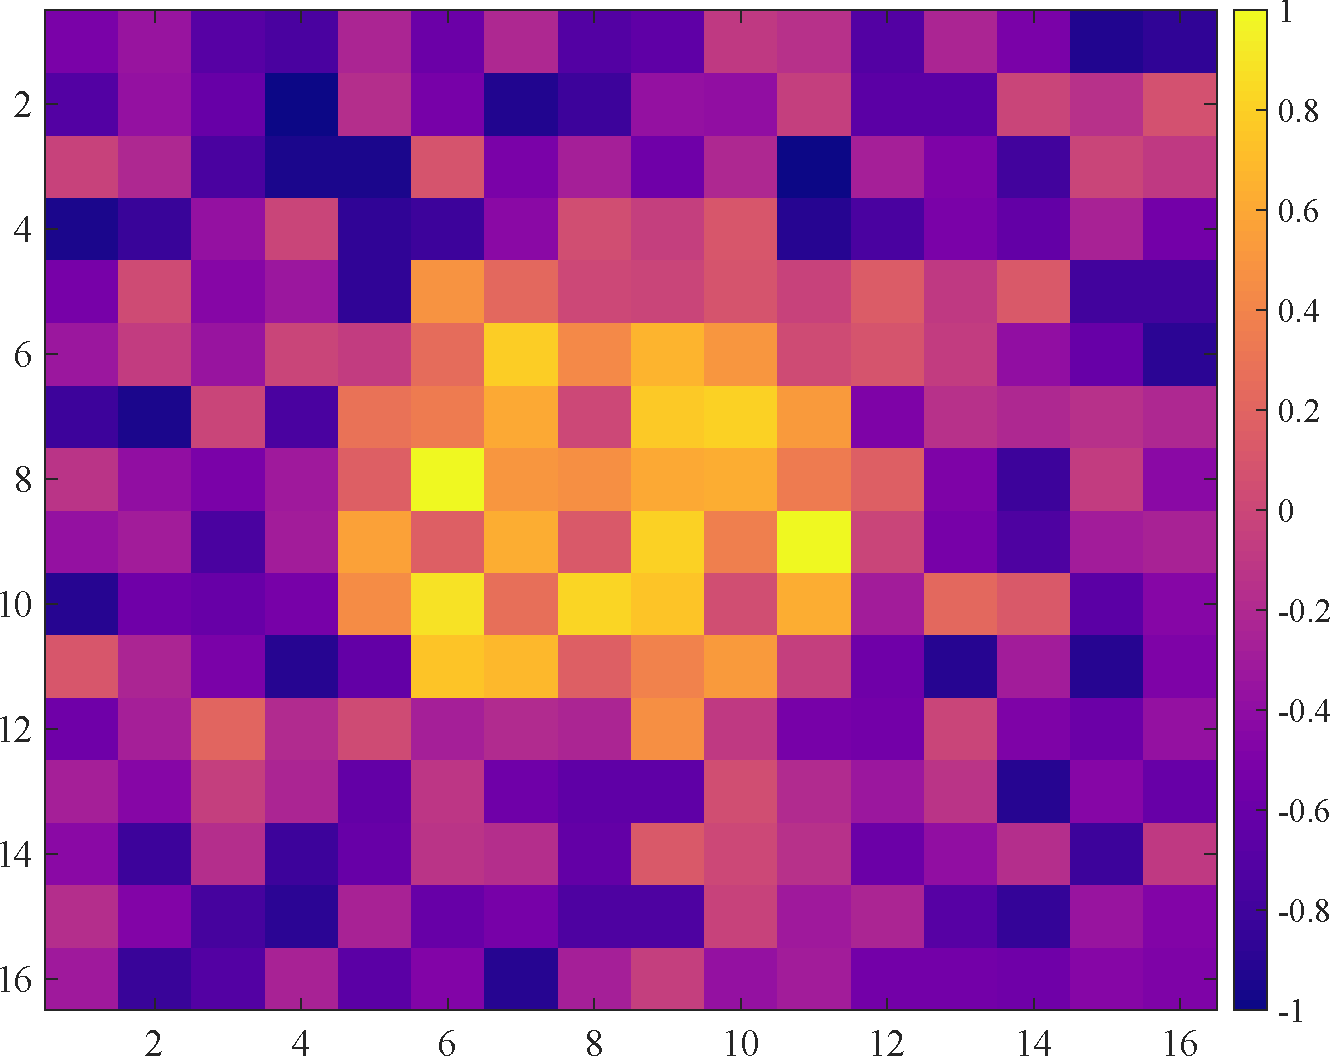
\includegraphics[width=0.45\linewidth]{Figures/Payload_ModulationSignal.pdf}
    }
    \caption{Reward function pipeline for the payload. The pipeline illustrates the raw \ac{dvs} events, the attention-based map, the normalized hidden layer activity during the initial training phase, and the reward signal calculated as the difference between the attention map and the hidden layer activity (\(r^{\text{H1}}(q)\)).}

    \label{fig:payloadRewardPipeline}
\end{figure}

Each grid cell in Figure~\ref{fig:payloadRewardPipeline}(d) shows the reward value assigned to the corresponding neuron in the payload detector repository of the first hidden layer. The spatial arrangement of these neurons follows the same layout as illustrated in Figure~\ref{fig:FiringActivityMatrix}, where each cell represents a specific neuron’s position within the repository grid.

Figure \ref{fig:AgentsRewardPipeline} shows an example of the reward function pipeline for the agent detector repository in the first hidden layer.

\begin{figure}[H]
    \centering
    \subfigure[Raw \ac{dvs} Events of the agents (Agent or \ac{scs} view)]{
        \includegraphics[width=0.45\linewidth]{Figures/Agents_RawDVS.pdf}
    }
    \hfill
    \subfigure[Attention Map (\(\mathcal{A}^{\text{Attention}}\))]{
        \includegraphics[width=0.45\linewidth]{Figures/Agents_AttentionFuzzyMap.pdf}
    }
    \vfill
    \subfigure[First Hidden Layer Activity (\(\mathbf{A}^{\text{H1}}\))]{
        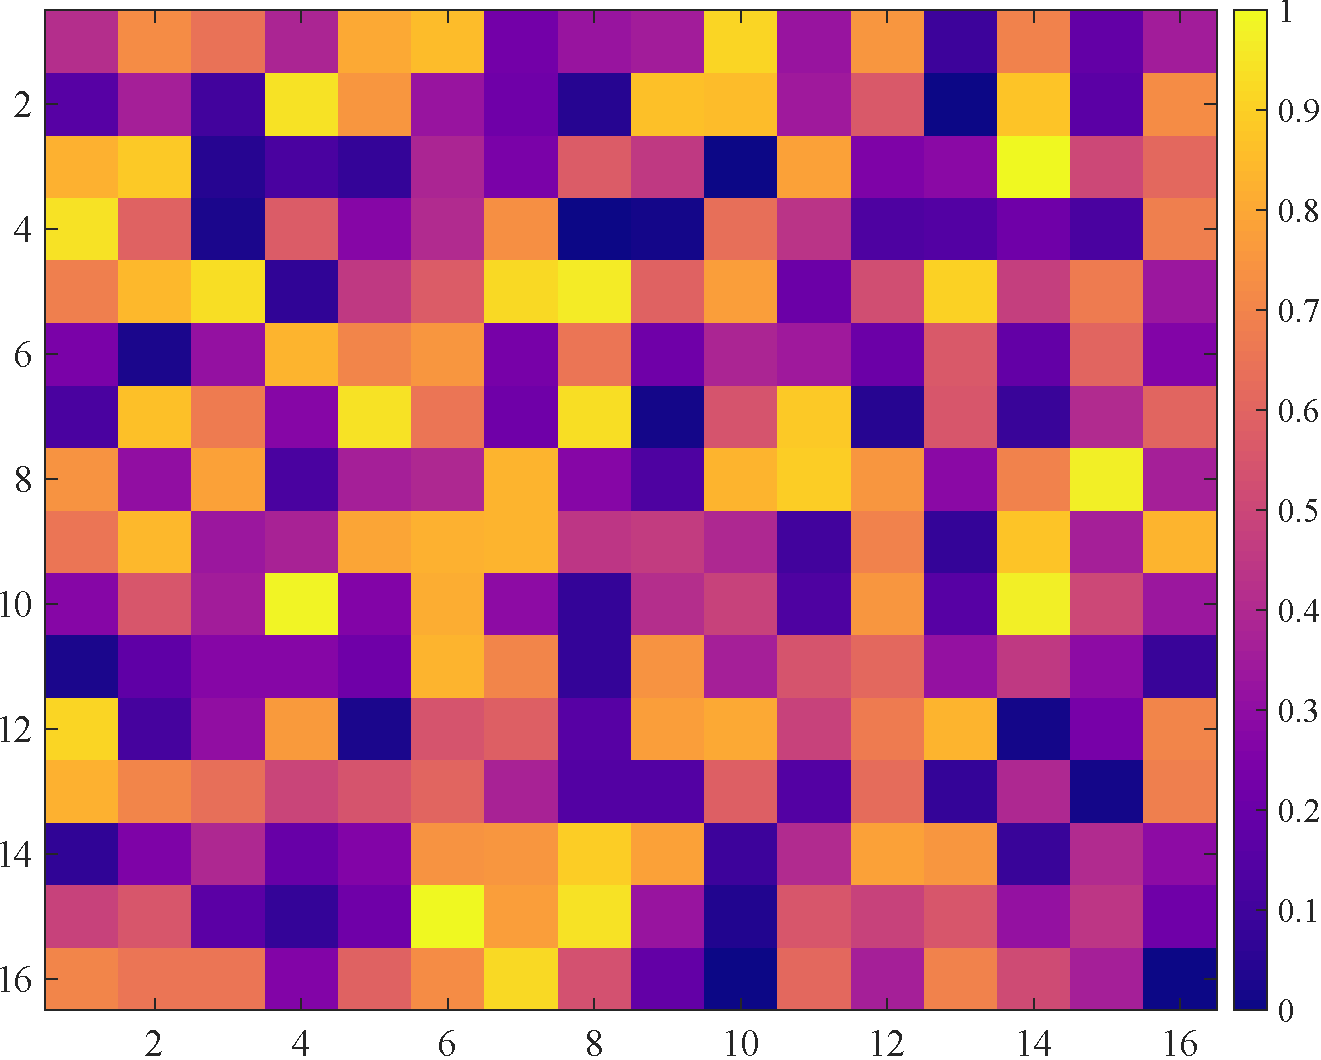
\includegraphics[width=0.45\linewidth]{Figures/Agents_HiddenLayerActivity.pdf}
    }
    \hfill
    \subfigure[First Hidden Layer Reward (\(r^{\text{H1}}\))]{
        \includegraphics[width=0.45\linewidth]{Figures/Agents_ModulationSignal.pdf}
    }
    \caption{Reward function pipeline for the agents. This pipeline demonstrates the raw \ac{dvs} events for multiple agents, the attention map, the hidden layer’s normalized activity, and the modulation signal computed for reward.}
    \label{fig:AgentsRewardPipeline}
\end{figure}

This design enables the first hidden layer to adaptively learn distinct environmental configurations (the spatial positions of the payload and nearby agents), using event-based attention and ensures stable convergence in layered \ac{snn} learning.











\paragraph{Numerical example (explicit Gaussian attention with $d_{kq}^2$ and $\gamma_{kq}$)}
Use an $8\times 8$ input grid and a $4\times 4$ first-hidden-layer grid (same as Figure~\ref{fig:FiringActivityMatrix}). Coordinates follow the code:
\[
x_k,y_k\in\{-1,\,-0.714,\,-0.429,\,-0.143,\,0.143,\,0.429,\,0.714,\,1\},
\qquad
x_q,y_q\in\{-1,\,-0.333,\,0.333,\,1\}.
\]

Set the attention scale to $\sigma_A=0.1$ and $\epsilon=0.001$. Let the time--averaged input activity (illustrated in Figure~\ref{fig:FiringActivityMatrix}) be
\[
\mathbf{A}^{\text{input}}=
\begin{bmatrix}
0&0&0&0&0&0&0&0\\
0&0.6&0.8&0.7&0&0&0&0\\
0&0.7&1.0&0.8&0&0&0&0\\
0&0.6&0.9&0.7&0&0&0&0\\
0&0&0&0&0&0.5&0.6&0.5\\
0&0&0&0&0.4&0.5&0.6&0.4\\
0&0&0&0&0.3&0.4&0.5&0.3\\
0&0&0&0&0&0&0&0
\end{bmatrix}.
\]

\begin{figure}[H]
    \centering
    \subfigure[Input activity matrix $(\mathbf{A}^{\text{input}})$ for numerical example of Gaussian attention computation.]{
        \includegraphics[width=0.45\linewidth]{Figures/Input activity matrix (8x8).pdf}
    }
    \hfill
    \subfigure[Hidden-layer centers of attention (queries) for numerical example of Gaussian attention computation.]{
        \includegraphics[width=0.45\linewidth]{Figures/Hidden neuron grid (4x4).pdf}
    }
    \caption{Numerical example setup for Gaussian attention computation in the first hidden layer. (a) shows the input activity matrix representing time-averaged firing rates from the input layer. (b) illustrates the spatial arrangement of hidden-layer neurons, each serving as a query point for attention calculation.}
    \label{fig:AttentionExample}
\end{figure}


\emph{Separable Gaussian weights along axes.}
For a $x_q$ in the first hidden layer, define the $8$-vector (one entry for each of the eight input columns)
\[
g_x(k\,|\,x_q)=\exp\!\Big(-\frac{(x_k-x_q)^2}{2\sigma_A^2}\Big),\qquad
2\sigma_A^2=0.02.
\]
Define the analogous 8-vector for the vertical axis, $g_y(r\,|\,y_q)$, which assigns a weight to each of the eight input rows centered at $y_q$. The full $8\times 8$ weight map for neuron $q$ is the outer product
% \[
% \gamma_{kq}=g_y(r\,|\,y_q)\,g_x(c\,|\,x_q),\qquad
% \gamma_{kq}=\gamma_{kq} \ \ \text{with }k\leftrightarrow(r,c).
% \]
\[
\gamma_{q}(r,c)=g_y(r\,|\,y_q)\,g_x(c\,|\,x_q),
\qquad
\gamma_{q}(r,c)\equiv \gamma_{kq}\ \text{with }k\leftrightarrow(r,c).
\]

The attention at $q$ is the normalized weighted average
\[
\mathcal{A}^{\text{Attention}}(q)=\frac{\sum_{r,c} \gamma_{kq}\,\mathbf{A}^{\text{input}}(r,c)}{\sum_{r,c} \gamma_{kq}+\epsilon}.
\]

\emph{Example 1: hidden neuron $q=(2,2)$ at $(x_q,y_q)=(-0.333,-0.333)$.}
Compute the axis weights:
\[
g_x(\cdot|-0.333)\approx [0.0000,\,0.0007,\,0.6308,\,0.1645,\,0.0000,\,0.0000,\,0.0000,\,0.0000],
\]
\[
g_y(\cdot|-0.333)\approx [0.0000,\,0.0007,\,0.6308,\,0.1645,\,0.0000,\,0.0000,\,0.0000,\,0.0000].
\]
Form $\gamma_{q}=g_y\,g_x^\top$. Non-negligible entries are the $2\times 2$ block on rows $3{:}4$, columns $3{:}4$ (Figure~\ref{fig:AttentionExampleWeights}(a)):
\[
\gamma_{q}(3,3)=0.6308\cdot 0.6308=0.398,\quad
\gamma_{q}(3,4)=0.6308\cdot 0.1645=0.104,\]
\[
\gamma_{q}(4,3)=0.1645\cdot 0.6308=0.104,\quad
\gamma_{q}(4,4)=0.1645\cdot 0.1645=0.027.
\]

\begin{figure}[H]
    \centering
    \subfigure[Gaussian weight map $(\gamma_{q})$.]{
        \includegraphics[width=0.45\linewidth]{Figures/Gaussian weight map.pdf}
    }
    \hfill
    \subfigure[Weighted input activity $(\gamma_{q} \odot \mathbf{A}^{\text{input}})$.]{
        \includegraphics[width=0.45\linewidth]{Figures/Weighted activity.pdf}
    }
    \caption{Attention weight computation for hidden neuron \( q = (2,2) \) at position \( (x_q, y_q) = (-0.333, -0.333) \). (a) shows the Gaussian weight map \( \gamma_{q} \) centered at the hidden neuron’s location. (b) illustrates the element-wise product of the weight map with the input activity matrix, highlighting the contributions to the attention calculation.}
    \label{fig:AttentionExampleWeights}
\end{figure}


The denominator (with $\epsilon$) is
\[
S_q=\sum_{r,c}\gamma_{q}(r,c)+\epsilon\approx(0.398+0.104+0.104+0.027)+0.001=0.635.
\]
The numerator uses the corresponding entries from $\mathbf{A}^{\text{input}}$:
\[
N_q=0.404\cdot 1.000+0.104\cdot 0.800+0.104\cdot 0.900+0.027\cdot 0.700=0.594.
\]
Hence 
\[
\mathcal{A}^{\text{Attention}}(2,2)=\frac{N_q}{S_q}= \frac{0.594}{0.635}=0.936.
\]

\emph{Example 2: hidden neuron $q=(2,1)$ at $(x_q,y_q)=(-1,-0.333)$.}
Here
\[
g_x(\cdot|-1)\approx[1.000,\,0.017,\,0.000,\,0.000,\,0.000,\,0.000,\,0.000,\,0.000]
\]
\[
g_y(\cdot|-0.333)\approx[0.000,\,0.001,\,0.636,\,0.163,\,0.000,\,0.000,\,0.000,\,0.000].
\]
Non-negligible weights sit on rows $3{:}4$ and columns $1{:}2$:
\[
\gamma_{q}(3,1)=0.636\cdot 1.000=0.636,,\quad
\gamma_{q}(3,2)=0.636\cdot 0.017=0.011,
\]
\[
\gamma_{q}(4,1)=0.163\cdot 1.000=0.163,,\quad
\gamma_{q}(4,2)=0.163\cdot 0.017=0.003.
\]
The denominator is $S_q\approx 0.636+0.011+0.163+0.003+0.001=0.814$.  
The numerator uses $\mathbf{A}^{\text{input}}(3,2)=0.7$ and $\mathbf{A}^{\text{input}}(4,2)=0.6$:
\[
N_q=0.011\cdot 0.7+0.003\cdot 0.6=0.009.
\]
Thus
\[
\mathcal{A}^{\text{Attention}}(2,1)=\frac{0.009}{0.814}=0.012.
\]

\emph{Example 3: hidden neuron $q=(3,3)$ at $(x_q,y_q)=(0.333,0.333)$.}
Axis weights are centered on columns $5{:}6$ and rows $5{:}6$:
\[
g_x(\cdot|0.333)\approx[0,0,0,0.163,0.636,0.000,0,0]
\quad\text{(nonzeros at col $5{:}6$ are $0.163,0.636$)},
\]
\[
g_y(\cdot|0.333)\approx[0,0,0,0.163,0.636,0,0,0]
\quad\text{(nonzeros at row $5{:}6$ are $0.163,0.636$)}.
\]
The four main weights are
\[
\gamma_{q}(5,5)=0.163\cdot 0.163=0.027,\;\;
\gamma_{q}(5,6)=0.163\cdot 0.636=0.104,\]
\[
\gamma_{q}(6,5)=0.636\cdot 0.163=0.104,\;\;
\gamma_{q}(6,6)=0.636\cdot 0.636=0.404.
\]
With $S_q\approx 0.404+0.104+0.104+0.027+0.001=0.640$ and
\[
N_q=0.027\cdot 0.000+0.104\cdot 0.500+0.104\cdot 0.400+0.404\cdot 0.500=0.296,
\]
one obtains
\[
\mathcal{A}^{\text{Attention}}(3,3)=\frac{0.296}{0.640}=0.463.
\]

\emph{Example 4: hidden neuron $q=(3,4)$ at $(x_q,y_q)=(1,0.333)$.}
Now $g_x$ sits on columns $7{:}8$ with weights $(0.017,\,1.000)$ and $g_y$ on rows $5{:}6$ with $(0.163,\,0.636)$. The four main weights are
\[
\gamma_{q}(5,7)=0.163\cdot 0.017=0.003,\ \ \gamma_{q}(5,8)=0.163\cdot 1.000=0.163,
\]
\[
\gamma_{q}(6,7)=0.636\cdot 0.017=0.011,\ \ \gamma_{q}(6,8)=0.636\cdot 1.000=0.636,
\]
so $S_q\approx 0.814$. With
\[
N_q=0.003\cdot 0.600+0.163\cdot 0.500+0.011\cdot 0.600+0.636\cdot 0.400=0.344,
\]
we get
\[
\mathcal{A}^{\text{Attention}}(3,4)=\frac{0.344}{0.814}=0.423.
\]

\emph{Assembling the $4\times4$ attention map.}
Repeating the above computation for all
$q \in \{1,\dots,4\}^2$ produces the attention values
\[
\mathcal{A}^{\text{Attention}} =
\begin{bmatrix}
0.000 & 0.014 & 0.000 & 0.000 \\
0.012 & 0.936 & 0.000 & 0.000 \\
0.000 & 0.000 & 0.463 & 0.423 \\
0.000 & 0.000 & 0.006 & 0.005
\end{bmatrix}.
\]

These values correspond to the normalized Gaussian attention centered at
the four-by-four hidden-layer coordinates and reflect the degree to which each
hidden neuron ``queries'' the spatio–temporal activity of the input grid.

\emph{Hidden-layer activities.}
Let the current hidden activities for the payload and agent detectors be
\[
\mathbf{A}^{\text{H1}}_{\text{payload}}=
\begin{bmatrix}
0.050 & 0.100 & 0.000 & 0.000\\
0.100 & 0.200 & 0.000 & 0.000\\
0.000 & 0.000 & 0.100 & 0.200\\
0.000 & 0.000 & 0.050 & 0.100
\end{bmatrix},
\qquad
\mathbf{A}^{\text{H1}}_{\text{agent}}=
\begin{bmatrix}
0.000 & 0.020 & 0.000 & 0.000\\
0.010 & 0.010 & 0.000 & 0.000\\
0.000 & 0.000 & 0.010 & 0.010\\
0.000 & 0.000 & 0.020 & 0.020
\end{bmatrix}.
\]

The activity matrices presented above are defined for the scenario when the \ac{alm} is turned off, which allows the first hidden layer to focus on detecting the payload. The small, nonzero values in the agent activity matrix occur because inhibition is not always perfect. Occasionally, some agent detector neurons (or payload detector neurons when the \ac{alm} is activated) may spike once or twice within the time window due to residual excitation or incomplete suppression.

\emph{Reward computation.}
Using the multiplicative reward definition
\(
r^{\text{H1}}(q) = \mathbf{A}^{\text{H1}}(q)\big(\mathcal{A}_{q}^{\text{Attention}} - \mathbf{A}^{\text{H1}}(q)\big),
\)
the elementwise rewards for the payload detector become
\[
r^{\text{H1}}_{\text{payload}}
=
\begin{bmatrix}
-0.0025 & -0.0086 & 0       & 0       \\
-0.0088 & 0.1472  & 0       & 0       \\
0       & 0       & 0.0363  & 0.0446  \\
0       & 0       & -0.0022 & -0.0095
\end{bmatrix}.
\]

With the updated agent-detector activity matrix, the corresponding reward values are
\[
r^{\text{H1}}_{\text{agent}}
=
\begin{bmatrix}
0        & -0.00012 & 0        & 0         \\
0.00002  & 0.00926  & 0        & 0         \\
0        & 0        & 0.00453  & 0.00413   \\
0        & 0        & -0.00028 & -0.00030
\end{bmatrix}.
\]

The combined reward vector is obtained by concatenating the
row-wise vectorizations of the two matrices,
\[
r^{\text{H1}}
=
\begin{bmatrix}
\operatorname{rowvec}\!\big(r^{\text{H1}}_{\text{payload}}\big) \\
\operatorname{rowvec}\!\big(r^{\text{H1}}_{\text{agent}}\big)
\end{bmatrix}
\in \mathbb{R}^{32\times 1}.
\]


Positive entries indicate that the attention-driven input estimate exceeds the neuron's present activity, leading to potentiation under the R-STDP rule. Negative values indicate that the neuron is currently overactive relative to the attended input and should undergo a reduction in synaptic efficacy. Since only one of the two repositories is active at any time because of lateral inhibition, only the corresponding reward matrix contributes to synaptic updates during each training iteration.


\subsubsection{Reward Function for the Second Hidden Layer}

Incoming \ac{dvs} events are represented as an image $E \in \{-1,0,+1\}^{N_e \times N_e}$, where each pixel encodes a negative, positive, or absent brightness change. The first hidden layer consists of two distinct neuron sections dedicated to payload detection and proximal agent detection, respectively. For each section, the time-averaged spiking activity is aggregated according to the activity-matrix construction rule illustrated in Figure~\ref{fig:FiringActivityMatrix}, resulting in two separate grid-based activity maps, $\mathbf{A}_{pay}^{\text{H1}}$ and $\mathbf{A}_{agt}^{\text{H1}}$, each of size $N_m \times N_m$.

Each grid cell in $\mathbf{A}_{pay}^{\text{H1}}$ and $\mathbf{A}_{agt}^{\text{H1}}$ corresponds to a fixed group of neurons in the respective section of the first hidden layer and represents the local firing-rate activity for that spatial region. These maps provide a spatial representation of the payload and proximal agents, indicating the extent to which the network associates each grid location with the presence of the corresponding object. The first hidden layer also incorporates a lateral inhibition mechanism, which ensures that only one of these two detection maps is active at any given time. When the payload detector neurons are active, the agent detector neurons are suppressed, and vice versa. Consequently, the instantaneous detection state of the network can be expressed as

\begin{equation}
    \mathbf{A}^{\text{H1}}_{\mathrm{det}} = \mathbf{A}_{pay}^{\text{H1}} + \mathbf{A}_{agt}^{\text{H1}},
    \label{eq:DetectionState}
\end{equation}
since at any given moment exactly one of the two terms on the right-hand side of~\eqref{eq:DetectionState} is nonzero.


To construct a binary activity-selection mask from the detection map, a Sigmoid function is applied element-wise,
\begin{equation}
    \mathbf{B}(i,j) =
    \frac{1}{1 + \exp\!\left[-\beta\left(\mathbf{A}^{\text{H1}}_{\mathrm{det}}(i,j)-\Upsilon\right)\right]},
\end{equation}
here, $\Upsilon$ denotes a soft threshold, and $\beta \gg 1$ determines the steepness of the transition. This operation converts the detection map into a logical mask that distinguishes active from inactive grid cells. Grid locations with nonzero and sufficiently large values of $\mathbf{A}^{\text{H1}}_{\mathrm{det}}(i,j)$ approach $1$, whereas locations with zero or negligible activity remain near $0$. Consequently, the resulting mask identifies spatial regions with high neural activity and suppresses regions that do not contribute to the detection process.


The \ac{dvs} produces events at the sensor resolution $N_e \times N_e$, corresponding to the native pixel grid of the event-based camera. In contrast, the activity maps generated by the entropy-based pooling input layer and the first hidden layer are defined on a coarser spatial grid of size $N_m \times N_m$, where each grid cell aggregates the activity of a fixed block of \ac{dvs} pixels according to the pooling rule described in Fig.~\ref{fig:FiringActivityMatrix}. Throughout this work, $N_e$ denotes the event (sensor) resolution, while $N_m$ refers to the pooled neural resolution. To apply the low-resolution activity-selection mask $\mathbf{B}$ to the original \ac{dvs} event image, the mask must be expanded from a size of $N_m \times N_m$ to the event resolution $N_e \times N_e$. Since the ratio $\kappa = N_e / N_m$ is an integer, this expansion is implemented using nearest-neighbor replication. Each entry of $\mathbf{B}$ is copied into a $\kappa \times \kappa$ block in the high-resolution grid, producing a mask that is spatially aligned with the original \ac{dvs} events. Formally, 
\begin{equation}
\mathcal{E}(\mathbf{B})
= B \otimes \mathbf{1}_{\kappa\times\kappa},
\qquad
(\mathcal{E}(\mathbf{B}))_{m,n}
= B_{\lceil m/\kappa \rceil,\;\lceil n/\kappa \rceil}.
\end{equation}
This operation ensures that every pixel $(m,n)$ in the enlarged mask $\mathcal{E}(\mathbf{B})$ inherits the value of the corresponding coarse mask element from $\mathbf{B}$, producing a properly aligned high event resolution binary mask. Finally, the upsampled mask is applied to the \ac{dvs} event frame to isolate only the currently detected object (payload or proximal agent),
\begin{equation}
E_{\mathrm{det}}
= E \odot \mathcal{E}(\mathbf{B}),
\end{equation}
where $\odot$ denotes element-wise multiplication. The resulting event image contains only the events emitted from the active target, with all other regions suppressed by the mask.


\begin{figure}[H]
    \centering
    \includegraphics[width=1\linewidth]{Figures/Second hidden Layer Reward Pipeline 1.pdf}
    \caption{The DVS event image is masked by the upsampled binary detection mask derived from the first hidden layer’s output, isolating events corresponding to the active object (payload or agent).}
    \label{fig:SecondLayerEventMasking}
\end{figure}

For the second hidden layer, the reward is designed to align synaptic updates with the spatial and temporal focus of the task. The temporal modulation is governed by the agent's \ac{alm} blinking period $T_{\text{ALM}}$, with oscillation frequency and angular frequency
\begin{equation}
f_{\text{osc}} = \frac{1}{T_{\text{ALM}}}, \qquad \omega = 2\pi f_{\text{osc}}.
\end{equation}

Let $G^{(e)} \in \mathbb{R}_+^{N_e\times N_e}$ be the Gaussian kernel sampled at the DVS resolution $N_e$, centered at the payload, with standard deviation $\sigma_g$. The scalar value that detects the motion direction (whether the object is getting closer to the center of the Gaussian envelope or not) is computed as

\begin{equation}
\mathcal{H} = \frac{1}{Z} \sum_{m=1}^{N_e}\sum_{n=1}^{N_e} E_{\mathrm{det}}^{(e)}(m,n) \, G^{(e)}(m,n,t) \in \mathbb{R}.
\end{equation}

The time-varying width and amplitude are

\begin{equation}
\sigma(t) = \sigma_0 + 0.5\sigma_0 \,\sin(\omega t), \qquad \alpha(t) = \cos(\omega t),
\end{equation}
yielding the oscillatory Gaussian envelope
\begin{equation}
G(x, y, t) = \alpha(t) \,\exp\!\left(-\frac{x^2 + y^2}{2\sigma(t)^2}\right), \quad (x, y) \in [-1, 1]^2.
\end{equation}
\begin{figure}[H]
    \centering
    \subfigure[Payload approaching the center results in positive \(\mathcal{H}\) value based on the 2D Gaussian function with higher standard deviation.]{
        \includegraphics[width=0.47\linewidth]{Figures/2D Gaussian Reward (Approaching the Center).pdf}
    }
    \hfill 
    \subfigure[Payload moving away from the center results in negative \(\mathcal{H}\) value based on the 2D Gaussian function with higher standard deviation.]{
        \includegraphics[width=0.47\linewidth]{Figures/2D Gaussian Reward (Going Away from the Center).pdf}
    }
    \caption{Payload motion direction detection using a 2D Gaussian reward function with higher standard deviation.}
    \label{fig:Positive2DGaussianReward}
\end{figure}

Figure~\ref{fig:Positive2DGaussianReward} illustrates how the motion direction of the payload is detected using a 2D Gaussian reward function with a higher standard deviation. When the payload moves closer to the center of the Gaussian envelope (\(G(x,y,t)\)), it results in a positive \(\mathcal{H}\) value, indicating favorable movement towards the target. Conversely, when the payload moves away from the center, it yields a negative \(\mathcal{H}\) value, signaling unfavorable movement away from the target.

\begin{figure}[H]
    \centering
    \subfigure[Neighboring agent approaching the center results in negative \(\mathcal{H}\) value based on the 2D Gaussian function with lower standard deviation.]{
        \includegraphics[width=0.47\linewidth]{Figures/Negative Reward - 2D Gaussian Reward (Approaching the Center).pdf}
    }
    \hfill
    \subfigure[Neighboring agent moving away from the center results in positive \(\mathcal{H}\) value based on the 2D Gaussian function with lower standard deviation.]{
        \includegraphics[width=0.47\linewidth]{Figures/Negative Reward - 2D Gaussian Reward (Going Away from the Center).pdf}
    }
    \caption{Neighboring agent motion direction detection using a 2D Gaussian reward function with lower standard deviation.}
    \label{fig:Negative2DGaussianReward}
\end{figure}

Figure~\ref{fig:Negative2DGaussianReward} demonstrates how the motion direction of a neighboring agent is detected using a 2D Gaussian reward function with a lower standard deviation. When the neighboring agent moves closer to the center of the Gaussian envelope (\(G(x,y,t)\)), it results in a negative \(\mathcal{H}\) value, indicating unfavorable movement towards the target. Conversely, when the neighboring agent moves away from the center, it yields a positive \(\mathcal{H}\) value, signaling favorable movement away from the target.

\begin{figure}[H]
    \centering
    \subfigure[The oscillatory Gaussian envelope when the \ac{alm} is off (payload's moves away from the center results in negative values).]{
        \includegraphics[width=0.47\linewidth]{Figures/Payload.pdf}
    }
    \hfill
    \subfigure[The oscillatory Gaussian envelope when the agent \ac{alm} is on (Agent's moves away from the center results in positive values).]{
        \includegraphics[width=0.47\linewidth]{Figures/Agent.pdf}
    }
    \caption{The oscillatory Gaussian envelope used to compute the motion direction signal $\mathcal{H}$ for reward modulation in the second hidden layer. The center can be \ac{scs} or the agent's \ac{dvs} center.}
    \label{fig:SecondLayerGaussianEnvelope}
\end{figure}

Figure~\ref{fig:SecondLayerGaussianEnvelope} illustrates the oscillatory Gaussian envelope used to compute the motion direction signal $\mathcal{H}$ for reward modulation in the second hidden layer. The envelope alternates between focusing on the payload and the agents based on which \ac{alm} is active. When the amplitude is positive, the envelope concentrates on the payload; when negative, it shifts focus to the agents. This dynamic modulation allows the network to adaptively learn from the relevant object based on the current task context. Getting close to the center of the Gaussian envelope can produce negative or positive $\mathcal{H}$ values depending on the phase of the oscillation, thereby influencing the reward signal accordingly.

Each agent is equipped with a planar inertial measurement unit (IMU) that measures the planar velocity
\(\mathbf{V} = [V_x, V_y]^\top\).
From this measurement, the instantaneous heading and normalized speed are computed as
\begin{equation}
\varphi = \operatorname{atan2}\left(V_y, V_x\right), \qquad
\bar{\mathcal{V}} = \frac{\|\mathbf{V}\|}{V_{\max}},
\end{equation}
where \(V_{\max}\) denotes the maximum admissible planar speed.

To obtain a population-based representation of velocity, the velocity space is discretized into an
\(N_g \times N_g\) grid (as shown in Figure~\ref{fig:FiringActivityMatrix} for the activity matrix).
Each grid cell corresponds to a fixed reference direction \((x_i, y_j)\), with
\(x_i, y_j \in [-1,1]\).
These reference points are expressed in normalized polar coordinates as
\begin{equation}
R_{ij} = \frac{\sqrt{x_i^2 + y_j^2}}{\sqrt{2}}, \qquad
\Theta_{ij} = \operatorname{atan2}\left(y_j, x_i\right).
\end{equation}

For a given velocity direction \(\varphi\), the angular mismatch between the reference direction
\(\Theta_{ij}\) and the actual heading is computed as follows:
\begin{equation}
\Delta\theta_{ij}
=
\operatorname{atan2}\!\left(
\sin(\Theta_{ij}-\varphi),\, \cos(\Theta_{ij}-\varphi)
\right).
\end{equation}

A separable Gaussian membership function is used to quantify the similarity between the current velocity
and each grid cell in terms of both speed and direction.
The radial and angular memberships are defined as
\begin{equation}
\mu_r(i,j)
=
\exp\!\left(-\frac{(R_{ij}-\bar{\mathcal{V}})^2}{2\sigma_r^2}\right),
\qquad
\mu_\theta(i,j)
=
\exp\!\left(-\frac{\Delta\theta_{ij}^2}{2\sigma_\theta^2}\right).
\end{equation}
Their product yields a velocity-aligned activity template,
\begin{equation}
\mathbf{M}_{ij}
=
\frac{\mu_r(i,j)\,\mu_\theta(i,j)}
{\max_{a,b} \mu_r(a,b)\,\mu_\theta(a,b)},
\end{equation}
which represents the desired neural activity pattern associated with the agent’s current velocity.
An opposite-direction template is obtained by rotating the heading by \(\pi\),
\begin{equation}
\widetilde{\mathbf{M}} = \mathbf{M}(\varphi + \pi).
\end{equation}


\begin{figure}
    \centering
    \subfigure[]{
        \includegraphics[width=0.47\linewidth]{Figures/Example for 2nd HL Velocity Reward (Positive).pdf}
    }
    \hfill
    \subfigure[]{
        \includegraphics[width=0.47\linewidth]{Figures/Example for 2nd HL Velocity Reward (Negative).pdf}
    }
    \caption{Velocity-aligned activity template \(\mathbf{M}\) (left) and opposite-direction template \(\widetilde{\mathbf{M}}\) (right) for an agent moving with heading \(\varphi = \pi/4\) and normalized speed \(\bar{\mathcal{V}} = 0.6\).}
    \label{fig:VelocityTemplates}
\end{figure}

Let \(\mathbf{A} \in [0,1]\) denote the normalized activity of neurons in the second hidden layer, defined as the
number of spikes emitted within a time window \(\Delta T\) divided by a maximum firing count.
The scalar reward signal \(\mathcal{H}\) is decomposed into positive and negative components as
\begin{equation}
\mathcal{H}_+ = \frac{\mathcal{H} + |\mathcal{H}|}{2}, \qquad
\mathcal{H}_- = \frac{|\mathcal{H}| - \mathcal{H}}{2},
\end{equation}
with \(\mathcal{H}_+ \ge 0\) representing reinforcement and \(\mathcal{H}_- \ge 0\) representing punishment.

Using this decomposition, the per-neuron reward assignment is defined as
\begin{equation}
L_i = \mathcal{H}_+ \mathbf{M}_i + \mathcal{H}_- \widetilde{\mathbf{M}}_i,
\end{equation}
such that positive reward reinforces neurons aligned with the current velocity direction,
while negative reward reinforces neurons encoding the opposite direction.

Finally, the reward-modulated learning signal applied to the second hidden layer is given by
\begin{equation}
r^{H2} =
\begin{cases}
\mathcal{H}_+(\mathbf{M}-\mathbf{A}) + \mathcal{H}_-(\widetilde{\mathbf{M}}-\mathbf{A}),
& \text{if } (V_x \neq 0)\ \lor\ (V_y \neq 0),\\[0.5ex]
0, & \text{if } V_x = 0 \ \land\ V_y = 0.
\end{cases}
\end{equation}
which is active only when the agent is in motion.
According to Figure~\ref{fig:VelocityTemplates}, this signal drives the neural activity toward the velocity-consistent template \(\mathbf{M}\) under positive
reward and toward the opposite template \(\widetilde{\mathbf{M}}\) under negative reward, while vanishing when
\(\mathcal{H}=0\).

\paragraph{Numerical example for the second hidden layer reward computation.}
We set $N_e=8$, $N_m=4$, hence the upsampling factor is $\kappa=N_e/N_m=2$.  
At the current instant the oscillatory envelope has amplitude $\alpha(t)=1$ (as given).  
Unless noted, all numbers are rounded to $3$ decimals.

\emph{Inputs.}
\[
E=
\begin{bmatrix}
0&0&0&0&0&0&0&0\\
0&1&-1&0&0&0&0&0\\
0&1&-1&0&0&0&0&0\\
0&0&0&0&0&0&0&0\\
0&0&0&0&0&1&1&0\\
0&0&0&0&-1&0&1&0\\
0&0&0&0&-1&-1&-1&0\\
0&0&0&0&0&0&0&0
\end{bmatrix},\quad
\mathbf{A}_{pay}^{\text{H1}}=
\begin{bmatrix}
0&0&0&0\\
0&0&0.1&0.1\\
0&0.1&0.8&0.7\\
0&0.3&0.7&0.5
\end{bmatrix},\quad
\mathbf{A}_{agt}^{\text{H1}}=\mathbf{0}_{4\times 4}.
\]
Thus $A_{\mathrm{det}}^{\text{H1}}=\mathbf{A}_{pay}^{\text{H1}}$.

\emph{Binarization and upsampling.}
With threshold $\Upsilon=0.3$ and steepness $\beta=10$,
\[
\mathbf{B}(i,j)=\frac{1}{1+\exp\!\big(-\beta(A_{\mathrm{det}}^{\text{H1}}(i,j)-\Upsilon)\big)}.
\]
For example $\mathbf{B}(3,3)=\frac{1}{1+\exp(-10(0.8-0.3))}=\frac{1}{1+e^{-5}}=0.993$.  
The full matrix is
\[
\mathbf{B}=
\begin{bmatrix}
0.047&0.047&0.047&0.047\\
0.047&0.047&0.119&0.119\\
0.047&0.119&0.993&0.982\\
0.047&0.500&0.982&0.881
\end{bmatrix}.
\]
Nearest–neighbor upsampling by $\kappa=2$ gives $\mathcal{E}(\mathbf{B})=\mathbf{B}\otimes\mathbf{1}_{2\times 2}$:
\[
\mathcal{E}(\mathbf{B})=
\begin{bmatrix}
0.047&0.047&0.047&0.047&0.047&0.047&0.047&0.047\\
0.047&0.047&0.047&0.047&0.047&0.047&0.047&0.047\\
0.047&0.047&0.047&0.047&0.119&0.119&0.119&0.119\\
0.047&0.047&0.047&0.047&0.119&0.119&0.119&0.119\\
0.047&0.047&0.119&0.119&0.993&0.993&0.982&0.982\\
0.047&0.047&0.119&0.119&0.993&0.993&0.982&0.982\\
0.047&0.047&0.500&0.500&0.982&0.982&0.881&0.881\\
0.047&0.047&0.500&0.500&0.982&0.982&0.881&0.881
\end{bmatrix}.
\]

\emph{Masked events.}
\[
E_{\mathrm{det}}=E\odot \mathcal{E}(\mathbf{B})=
\begin{bmatrix}
0&0&0&0&0&0&0&0\\
0&0.047&-0.047&0&0&0&0&0\\
0&0.047&-0.047&0&0&0&0&0\\
0&0&0&0&0&0&0&0\\
0&0&0&0&0&0.993&0.982&0\\
0&0&0&0&-0.993&0&0.982&0\\
0&0&0&0&-0.982&-0.982&-0.881&0\\
0&0&0&0&0&0&0&0
\end{bmatrix}.
\]

\emph{Gaussian kernel and scalar reward.}
We sample a centered Gaussian kernel $G^{(e)}$ on the $8\times 8$ grid with coordinates
$\{-0.875,-0.625,-0.375,-0.125,0.125,0.375,0.625,0.875\}$ on each axis and width $\sigma_g=0.6$:
\[
G^{(e)}(m,n)=\exp\!\Big(-\frac{x^2+y^2}{2\sigma_g^2}\Big).
\]
This yields
\[
\mathbf{G}^{(e)}=
\begin{bmatrix}
0.119&0.201&0.284&0.338&0.338&0.284&0.201&0.119\\
0.201&0.338&0.478&0.569&0.569&0.478&0.338&0.201\\
0.284&0.478&0.677&0.805&0.805&0.677&0.478&0.284\\
0.338&0.569&0.805&0.958&0.958&0.805&0.569&0.338\\
0.338&0.569&0.805&0.958&0.958&0.805&0.569&0.338\\
0.284&0.478&0.677&0.805&0.805&0.677&0.478&0.284\\
0.201&0.338&0.478&0.569&0.569&0.478&0.338&0.201\\
0.119&0.201&0.284&0.338&0.338&0.284&0.201&0.119
\end{bmatrix},\qquad
Z=\sum_{m,n}\mathbf{G}^{(e)}(m,n)=29.761.
\]
The motion-direction signal is
\[
\mathcal{H}=\frac{1}{Z}\sum_{m,n} E_{\mathrm{det}}(m,n)\,\mathbf{G}^{(e)}(m,n).
\]
Only $11$ positions are nonzero,
\[
\small
\begin{array}{rcl}
(2,2):\ 0.047\cdot 0.338=0.016,&\quad& (2,3):\ -0.047\cdot 0.478=-0.023,\\
(3,2):\ 0.047\cdot 0.478=0.023,&\quad& (3,3):\ -0.047\cdot 0.677=-0.032,\\
(5,6):\ 0.993\cdot 0.805=0.800,&\quad& (5,7):\ 0.982\cdot 0.569=0.559,\\
(6,5):\ -0.993\cdot 0.805=-0.800,&\quad& (6,7):\ 0.982\cdot 0.478=0.469,\\
(7,5):\ -0.982\cdot 0.569=-0.559,&\quad& (7,6):\ -0.982\cdot 0.478=-0.470,\\
(7,7):\ -0.881\cdot 0.338=-0.298,&&
\end{array}
\]
whose sum is $-0.314$. Therefore
\[
\mathcal{H}=\frac{-0.314}{29.761}=-0.011,\qquad
\mathcal{H}_{+}=0,\ \ \mathcal{H}_{-}=\frac{|\mathcal{H}|-\mathcal{H}}{2}=0.011.
\]
which means that the payload is moving away from the center of the Gaussian envelope and the agants receive negative reward.

\emph{Velocity encoding and memberships.}
Take $\mathbf{V}=[0.6,\,0.2]^\top$ (illustrative), $V_{\max}=1$. Then
\[
\varphi=\operatorname{atan2}(0.2,0.6)=0.322~\mathrm{rad},\qquad
\bar{\mathcal{V}}=\min(\|\mathbf{V}\|/V_{\max},1)=0.632.
\]
On a $3\times 3$ grid with $(x_i,y_j)\in\{-1,0,1\}^2$, define
$R_{ij}=\sqrt{x_i^2+y_j^2}/\sqrt{2}$ and
$\Theta_{ij}=\operatorname{atan2}(y_j,x_i)$ (set $\Theta_{2,2}=\varphi$ at the origin).
With $\sigma_r=0.3$, $\sigma_\theta=0.6$,
\[
\mu_r=
\begin{bmatrix}
0.472&0.970&0.472\\
0.970&0.108&0.970\\
0.472&0.970&0.472
\end{bmatrix},\quad
\mu_\theta=
\begin{bmatrix}
0.000&0.007&0.182\\
0.000&1.000&0.866\\
0.003&0.115&0.742
\end{bmatrix}.
\]
Normalize \(\mathbf{M}_{ij}=\mu_r(i,j)\mu_\theta(i,j)/\max_{a,b}\mu_r(a,b)\mu_\theta(a,b)\) and form the opposite-direction map \(\widetilde{\mathbf{M}}=\mathbf{M}(\varphi+\pi)\):
\[
\mathbf{M}=
\begin{bmatrix}
0.000&0.008&0.102\\
0.000&0.129&1.000\\
0.002&0.132&0.417
\end{bmatrix},\qquad
\widetilde{\mathbf{M}}=
\begin{bmatrix}
0.417&0.132&0.002\\
1.000&0.000&0.000\\
0.102&0.008&0.000
\end{bmatrix}.
\]

\emph{Per–neuron reward and signed credit.}
Let the normalized second–layer activities be
\[
\mathbf{A}=
\begin{bmatrix}
0.100&0.200&0.300\\
0.400&0.500&0.200\\
0.100&0.300&0.600
\end{bmatrix}.
\]
Since $\mathcal{H}<0$,
\[
r^{H2}=\mathcal{H}_+(\mathbf{M}-\mathbf{A})+\mathcal{H}_-(\widetilde{\mathbf{M}}-\mathbf{A})=0.011\,(\widetilde{\mathbf{M}}-\mathbf{A}),
\]
so
\[
r^{H2}=
\begin{bmatrix}
\phantom{-}0.003&-0.001&-0.003\\
\phantom{-}0.006&-0.005&-0.002\\
\phantom{-}0.000&-0.003&-0.006
\end{bmatrix}.
\]

The shape of this reward (matrix form) follows the same rule as Figure~\ref{fig:FiringActivityMatrix}, and each array shows the reward value for each associated neuron. 

\emph{Interpretation.}
The masked events and Gaussian envelope yield a small \emph{negative} motion signal ($-0.011$), so learning pushes activity toward the \emph{opposite} velocity map \(\widetilde{\mathbf{M}}\): cells aligned with \(\varphi+\pi\) are encouraged (positive entries in \(\mathbf{L}\)), while currently overactive cells are suppressed by the negative entries of \(\dot{\mathbf{W}}\).

\subsubsection{Output Layer Reward Computation Based on Directional Error}


The output layer consists of four neurons that generate thrust commands along the Cartesian
directions \(\pm X\) and \(\pm Y\).
The role of the reward at this layer is to align the generated action with a commanded
motion direction provided by the preceding (second hidden) layer.

The second hidden layer encodes motion direction using a population of neurons whose
preferred directions are uniformly distributed over the unit circle.
Each neuron responds most strongly when the motion direction matches its preferred
orientation.
Let \(\mu_k \in [0,2\pi)\) denote the preferred direction of the \(k\)-th neuron.
The activity of each neuron is quantified by a binned spike count \(w_k \ge 0\), defined as
the total number of spikes emitted within a fixed temporal window of duration
\(\Delta T = 10~\mathrm{ms}\).
This temporal binning converts discrete spike trains into a nonnegative scalar activity
that can be used for population-level decoding.

The commanded motion direction is extracted from this population activity using a
circular mean.
Specifically, the population is interpreted as a set of weighted unit vectors oriented
along \(\mu_k\), and their vector sum is computed as
\begin{equation}
C = \sum_k w_k \cos(\mu_k), \qquad
S = \sum_k w_k \sin(\mu_k).
\end{equation}
The commanded direction is then given by the angle of the resulting vector,
\begin{equation}
\theta_{\mathrm{cmd}} = \operatorname{atan2}(S,\,C),
\end{equation}
which corresponds to the circular mean of the population activity and yields a direction.


The output layer consists of four neurons associated with thrust along the negative and
positive \(X\) and \(Y\) directions.
Let \(a_x\) and \(a_y\) denote the net thrust components along the \(X\) and \(Y\) axes,
obtained as the difference between the spike activities of neurons encoding opposite
directions and averaged over a \(50~\mathrm{ms}\) window.
These components define the instantaneous action vector, \(\mathbf{a} = (a_x, a_y)\). The direction of this vector represents the action executed by the network.
Since only the direction of the action is relevant for reward assignment, explicit
normalization of \(\mathbf{a}\) is not required; the angular information is extracted
directly via
\begin{equation}
\theta_{\mathrm{act}} = \operatorname{atan2}(a_y,\; a_x).
\end{equation}

To assess directional consistency, the commanded and executed directions are compared
through their trigonometric components.
The discrepancies along the \(X\) and \(Y\) axes are defined as
\begin{equation}
\Delta_c = \cos(\theta_{\mathrm{cmd}}) - \cos(\theta_{\mathrm{act}}), \qquad
\Delta_s = \sin(\theta_{\mathrm{cmd}}) - \sin(\theta_{\mathrm{act}}).
\end{equation}
These quantities measure the mismatch between the desired and actual motion directions in
each Cartesian dimension.

Based on these discrepancies, the per-neuron rewards for the output layer are assigned as
\begin{equation}
r_{X^-} = \Delta_c, \qquad
r_{X^+} = -\Delta_c, \qquad
r_{Y^-} = \Delta_s, \qquad
r_{Y^+} = -\Delta_s.
\end{equation}
This reward structure reinforces neurons whose activity contributes to reducing the
directional error between the commanded motion (decoded from the second hidden layer) and
the executed action, while suppressing neurons that drive motion in the opposite direction.

% \subsubsection{Output Layer Reward Computation Based on Directional Error}

% The final output layer of the network generates four motor control signals, corresponding to the application of force in the $\pm X$ and $\pm Y$ directions in a planar environment. The purpose of the reward function is to adjust the firing rates of these output neurons such that the resulting acceleration aligns with the commanded velocity direction produced by the second hidden layer. This second hidden layer outputs an $N_g \times N_g$ activity map $A_2^{hidden} \in [0,1]^{N_g\times N_g}$, representing a fuzzy encoding of the desired velocity direction.

% The reward computation proceeds in four main steps. First, the reference velocity direction is decoded from the activity map. A Cartesian grid is defined over the range $[-1,1] \times [-1,1]$:
% \begin{equation}
% x_{ij},\, y_{ij} \in [-1,1], \quad i,j \in \{1,\dots,N_g\},
% \end{equation}
% and the radial distance is computed as
% \begin{equation}
% r_{ij} = \sqrt{x_{ij}^2 + y_{ij}^2} + \varepsilon,
% \end{equation}
% where $\varepsilon$ is a small constant to avoid division by zero. The local unit vectors at each grid cell are
% \begin{equation}
% e_x(i,j) = \frac{x_{ij}}{r_{ij}}, \qquad e_y(i,j) = \frac{y_{ij}}{r_{ij}}.
% \end{equation}
% Here, $e_x$ and $e_y$ define the unit vector field pointing radially outward from the origin.

% The activity map $A_2^{hidden}$ is first normalized to form a weighting distribution:
% \begin{equation}
% \lambda(i,j) = \frac{\max\left(A_2^{hidden}(i,j),\, 0\right)}{\sum_{p=1}^{N_g}\sum_{q=1}^{N_g} \max\left(A_2^{hidden}(p,q),\, 0\right) + \varepsilon}.
% \end{equation}
% The reference velocity vector is then computed as the projection of the activity map onto the local unit vector field:
% \begin{equation}
% \mathbf{V}_{\mathrm{ref}} = 
% \begin{bmatrix}
% \sum_{i=1}^{N_g}\sum_{j=1}^{N_g} \lambda(i,j)\, e_x(i,j) \\[4pt]
% \sum_{i=1}^{N_g}\sum_{j=1}^{N_g} \lambda(i,j)\, e_y(i,j)
% \end{bmatrix}.
% \end{equation}
% This vector is normalized to unit length:
% \begin{equation}
% \hat{\mathbf{V}}_{\mathrm{ref}} = \frac{\mathbf{V}_{\mathrm{ref}}}{\|\mathbf{V}_{\mathrm{ref}}\| + \varepsilon}.
% \end{equation}

% In the second step, the measured velocity vector \(\mathbf{V}_{\mathrm{meas}}\) is obtained from the IMU by numerical integration of the measured accelerations. The measured velocity direction is then
% \begin{equation}
% \hat{\mathbf{V}}_{\mathrm{meas}} = \frac{\mathbf{V}_{\mathrm{meas}}}{\|\mathbf{V}_{\mathrm{meas}}\| + \varepsilon}.
% \end{equation}

% In the third step, the signed component-wise directional error is computed as
% \begin{equation}
% \mathbf{e} = \hat{\mathbf{V}}_{\mathrm{ref}} - \hat{\mathbf{V}}_{\mathrm{meas}}.
% \end{equation}
% This error is optionally compressed using the hyperbolic tangent \(\tanh(\mathbf{e})\) to avoid excessive updates, which preserves the sign while bounding the magnitude to approximately $\pm 1$.

% In the final step, the two error components $e_x$ and $e_y$ are mapped to the four output-neuron rewards:
% \begin{equation}
% r_{X^+} = e_x, \quad r_{X^-} = -e_x, \quad r_{Y^+} = e_y, \quad r_{Y^-} = -e_y.
% \end{equation}
% Positive values of $r_{X^+}$ or $r_{Y^+}$ encourage increased firing of the corresponding neuron to push in the positive $X$ or $Y$ direction, whereas positive values of $r_{X^-}$ or $r_{Y^-}$ encourage firing in the opposite direction to reduce the error. All rewards are clipped to the range $[-1,1]$ to ensure numerical stability.

% This formulation ensures that the output layer learns to generate low-level motor commands that minimize the difference between the commanded velocity direction from the second hidden layer and the actual velocity direction measured by the IMU.

\subsubsection{Weight Update using \ac{stdp}}
\label{subsubsec:stdp_weight_update}

Simultaneous plasticity across multiple layers in spiking neural networks leads to unstable learning~\cite{wilmes2023dendrites}. This occurs because downstream synapses adapt while upstream feature representations are still evolving. Accordingly, prior work in \ac{stdp}, biologically inspired deep SNNs, and hierarchical reinforcement learning employs mechanisms that delay, gate, or attenuate learning signals until lower-level representations stabilize~\cite{fremaux2016neuromodulated}. 

To ensure consistent hierarchical learning, synaptic plasticity in each layer is modulated
by the convergence state of the preceding layer.
Let \(r^{\ell-1}_i\) denote the instantaneous reward signal associated with neuron \(i\) in
layer \(\ell-1\).
The overall activity-dependent instability of that layer is summarized by the scalar
measure
\begin{equation}
\mathcal{R}^{\ell-1} = \max_i \, |r^{\ell-1}_i|,
\end{equation}
which captures the largest magnitude of reward-driven fluctuations within the layer.

Since the reward signals \(r^{\ell-1}_i\) are bounded by construction, the quantity
\(\mathcal{R}^{\ell-1}\) is finite and nonnegative.
Using this measure, the effective reward driving learning in layer \(\ell\) is defined as
\begin{equation}
r^{\ell}_{\mathrm{eff}}
=
r^{\ell} \exp\!\left(-a_L \, \mathcal{R}^{\ell-1}\right),
\label{effectiveReward}
\end{equation}
where \(a_L > 0\) is a tunable damping coefficient.

This exponential modulation suppresses downstream plasticity when the preceding layer exhibits large reward fluctuations, indicating ongoing adaptation. As learning in layer \(\ell-1\) stabilizes and its weight adjustment becomes negligible ($|r^{\ell-1}_i|$ goes to zero), the \(\mathcal{R}^{\ell-1}\) decreases, enabling gradual adaptation in layer \(\ell\).


\begin{figure}[H]
    \centering
    \includegraphics[width=0.65\textwidth]{figures/Weight Update.pdf}
    \caption{Schematic of the per-layer R-STDP weight update. The eligibility trace is calculated based on the firing rate of the neurons in layer \(\ell\) and \(\ell+1\). The per-neuron reward (\(r_q\)) is computed based on the layer-specific reward functions. The weight update is obtained by multiplying the eligibility trace by the per-neuron reward.}
    \label{fig:weight_update}
\end{figure}

As shown in Figure~\ref{fig:weight_update}, the network is partitioned into layers using indices \(\{\ell=1,\dots,L-1\}\). For each layer \(\ell\), let \(\mathcal{J}_\ell\) be the set of presynaptic indices and \(\mathcal{I}_{\ell+1}\) the set of postsynaptic indices ($h, i,$ and $j$ in Layer $l$). Denote by \(\mathbf{C}^{(\ell)}(t)\in\mathbb{R}^{|\mathcal{I}_{\ell+1}|\times|\mathcal{J}_\ell|}\) the eligibility (credit–assignment) matrix produced by the \ac{stdp} kernel from pre– and post–spike timings up to time \(t\). In continuous time an admissible form is
\begin{equation}
\dot{\mathbf{C}^l}(t) = -\frac{1}{\tau_c}\mathbf{C}^l(t) + \mathbf{STDP}(\tau) \delta(t - \mathbf{T}^l)
\end{equation}
where, \(\tau_c\) is the constant for the decay of \(\mathbf{C}^l(t)\), the \(\tau\) is the spike time difference between pre- and post-synaptic neurons (e.g., $h$ and $q$ in Figure~\ref{fig:weight_update}), and \(\mathbf{T}^l\) is the matrix that shows the firing times of pre- and post-synaptic neurons. In discrete implementation this eligibility is maintained internally and sampled at update times; the weight rule below treats \(\mathbf{C}^{(\ell)}(t)\) as known.

Per–neuron rewards computed on the postsynaptic side of each layer. The instantaneous, gated R-STDP update for layer \(\ell\) is then
\begin{equation}
\Delta\mathbf{W}^{(\ell)}(t)\;=\; \boldsymbol{r}^{(\ell)}_{\mathrm{eff}}(t) \circ \mathbf{C}^{(\ell)}(t),
\label{eq:layer_update}
\end{equation}
where \(\circ\) denotes element–wise multiplication. 

% \subsubsection{Per--Neuron, Cross--Resolution Federated Aggregation}

% Fix a layer index $\ell$. Let the set of clients be $\mathcal{Z}$ and index clients by $\mathcal{X}\in\mathcal{Z}$. Client $\mathcal{X}$ has $M^{[\mathcal{X}]}$ presynaptic and $\mathcal{P}^{[\mathcal{X}]}$ postsynaptic neurons (so each postsynaptic neuron in this layer receives $M^{[\mathcal{X}]}$ incoming synapses). For each postsynaptic neuron $h\in\{1,\dots,\mathcal{P}^{[\mathcal{X}]}\}$, the local R--STDP rule produces a column of weight updates
% \begin{equation}
% \boldsymbol{\Delta W}^{[\mathcal{X}]}_{\ell,h}\in\mathbb{R}^{\,M^{[\mathcal{X}]}}\!,
% \end{equation}
% whose $k$-th entry is the incremental change $\Delta W_{\ell}(k,h)$ for the synapse from presynaptic index $k$ to neuron $h$. Each neuron transmits only its weight--update column $\boldsymbol{\Delta W}^{[\mathcal{X}]}_{\ell,h}$ (no eligibility trace or reward is exchanged).

% To compare heterogeneous presynaptic widths across clients, introduce linear compression/expansion operators
% \begin{equation}
% \boldsymbol{\Phi}^{[\mathcal{X}]}:\mathbb{R}^{\,M^{[\mathcal{X}]}}\!\to\mathbb{R}^{\,d_{\mathrm{lat}}},\qquad
% \boldsymbol{\Psi}^{[\mathcal{X}]}:\mathbb{R}^{\,d_{\mathrm{lat}}}\!\to\mathbb{R}^{\,M^{[\mathcal{X}]}}\!,
% \end{equation}
% chosen as a truncated Discrete Cosine Transform (DCT--II). For a one--dimensional presynaptic width $M^{[\mathcal{X}]}$, define the orthonormal DCT--II matrix
% \begin{equation}
% \big[\mathbf{C}^{[\mathcal{X}]}\big]_{k,n}
% =\alpha_k\,\cos\!\Big(\frac{\pi}{M^{[\mathcal{X}]}}\Big(n+\tfrac{1}{2}\Big)k\Big),
% \quad
% \alpha_0=\sqrt{\tfrac{1}{M^{[\mathcal{X}]}}},\ \ 
% \alpha_k=\sqrt{\tfrac{2}{M^{[\mathcal{X}]}}}\ (k\ge 1),
% \end{equation}
% with $k,n\in\{0,\dots,M^{[\mathcal{X}]}-1\}$. Let $\mathbf{P}_{d}$ select the first $d_{\mathrm{lat}}$ low--frequency rows (in increasing frequency order). Then
% \begin{equation}
% \boldsymbol{\Phi}^{[\mathcal{X}]}=\mathbf{P}_{d}\,\mathbf{C}^{[\mathcal{X}]}, 
% \qquad
% \boldsymbol{\Psi}^{[\mathcal{X}]}=\big(\mathbf{C}^{[\mathcal{X}]}\big)^{\!\top}\mathbf{P}_{d}^{\top}.
% \end{equation}
% Thus the latent
% \(
% \boldsymbol{\mu}^{[\mathcal{X}]}_{\ell,h}=\boldsymbol{\Phi}^{[\mathcal{X}]}\boldsymbol{\Delta W}^{[\mathcal{X}]}_{\ell,h}\in\mathbb{R}^{\,d_{\mathrm{lat}}}
% \)
% keeps the lowest $d_{\mathrm{lat}}$ DCT coefficients (a compact summary of the smooth/topographic component of the update). Reconstruction
% \(
% \widehat{\boldsymbol{\Delta W}}^{[\mathcal{X}]}_{\ell,h}
% =\boldsymbol{\Psi}^{[\mathcal{X}]}\breve{\boldsymbol{\mu}}^{[\mathcal{X}]}_{\ell,h}
% \)
% is the corresponding inverse DCT with zero--padding of discarded modes. Because $\mathbf{C}^{[\mathcal{X}]}$ is orthonormal, Parseval's identity implies that the truncation error equals the energy of the omitted high--frequency coefficients; one may choose $d_{\mathrm{lat}}$ via an energy--retention criterion
% \[
% \|\boldsymbol{\mu}^{[\mathcal{X}]}_{\ell,h}\|_2^2 \;\ge\; (1-\varepsilon)\,\|\boldsymbol{\Delta W}^{[\mathcal{X}]}_{\ell,h}\|_2^2,
% \]
% for a small tolerance $\varepsilon\in(0,1)$. The per--vector complexity is $O\!\big(M^{[\mathcal{X}]}\log M^{[\mathcal{X}]}\big)$ and requires no training. If the presynaptic map is two--dimensional, the same construction uses the separable 2D DCT $\mathbf{C}_y\otimes\mathbf{C}_x$.

% \paragraph{Neuron signatures and similarity kernel.}
% For each client $\mathcal{X}$ and postsynaptic neuron $h$, we attach a short vector
% $\boldsymbol{\pi}^{[\mathcal{X}]}_{h}\in\mathbb{R}^{\,p_{\mathrm{sig}}}$ that places this neuron
% in a common coordinate system so that neurons from different clients can be compared.
% We give two practical constructions.

% \emph{(A) Data--driven receptive--field summary.}
% Assume the presynaptic sites are arranged on a known grid with coordinates
% $\{\mathbf{r}_k\}_{k=1}^{M^{[\mathcal{X}]}}\subset[0,1]^d$ (e.g., $d=1$ for a line or $d=2$ for a 2D map),
% and let $\Delta W^{[\mathcal{X}]}_{\ell,h}(k)$ be the update on the synapse from site $k$ to neuron $h$.
% Define normalized, nonnegative weights
% \[
% p_k \;=\; \frac{\big|\Delta W^{[\mathcal{X}]}_{\ell,h}(k)\big|}{\sum_{m=1}^{M^{[\mathcal{X}]}}\big|\Delta W^{[\mathcal{X}]}_{\ell,h}(m)\big| + \varepsilon},
% \qquad \varepsilon>0 \text{ small},\quad \sum_k p_k=1,
% \]
% the \emph{centroid}
% \[
% \mathbf{c}^{[\mathcal{X}]}_{h} \;=\; \sum_{k=1}^{M^{[\mathcal{X}]}} p_k\,\mathbf{r}_k \in[0,1]^d,
% \]
% and a scalar \emph{spread}
% \[
% \delta^{[\mathcal{X}]}_{h} \;=\; \Big(\sum_{k=1}^{M^{[\mathcal{X}]}} p_k \,\|\mathbf{r}_k-\mathbf{c}^{[\mathcal{X}]}_{h}\|_2^2\Big)^{1/2}.
% \]
% We then set $\boldsymbol{\pi}^{[\mathcal{X}]}_{h}=\big[\,\mathbf{c}^{[\mathcal{X}]}_{h};\,\delta^{[\mathcal{X}]}_{h}\,\big]$, so $p_{\mathrm{sig}}=d+1$.
% This summarizes where the update is concentrated (centroid) and how wide it is (spread).

% \emph{(\mathbf{B}) Topographic index (no explicit grid).}
% If only the postsynaptic order is known, use the normalized index
% $\tau^{[\mathcal{X}]}_{h}=(h-\tfrac{1}{2})/\mathcal{P}^{[\mathcal{X}]} \in (0,1)$ and set
% $\boldsymbol{\pi}^{[\mathcal{X}]}_{h}=\tau^{[\mathcal{X}]}_{h}$ (so $p_{\mathrm{sig}}=1$).
% This places neurons uniformly along a line, which is often sufficient.

% To compare two neurons we use a positive kernel
% $\mathcal{K}:\mathbb{R}^{p_{\mathrm{sig}}}\times\mathbb{R}^{p_{\mathrm{sig}}}\to\mathbb{R}_{+}$.
% We adopt the Gaussian kernel
% \[
% \mathcal{K}(\mathbf{a},\mathbf{b})=\exp\!\Big(-\tfrac{\|\mathbf{a}-\mathbf{b}\|_2^2}{2\varsigma^{2}}\Big),
% \]
% where the \emph{bandwidth} $\varsigma>0$ controls how quickly similarity decays with distance in signature space:
% small $\varsigma$ makes each neuron borrow only from very close matches (sharp assignment),
% while large $\varsigma$ blends information from a broader neighborhood (soft assignment).

% Define the row--stochastic \emph{transport} from client $\mathcal{X}$ to client $\mathcal{Y}$ by
% \begin{equation}
% \Pi^{(\mathcal{Y}\gets \mathcal{X})}_{h j}
% = \frac{\mathcal{K}\!\big(\boldsymbol{\pi}^{[\mathcal{Y}]}_{h},\,\boldsymbol{\pi}^{[\mathcal{X}]}_{j}\big)}
% {\sum_{j'} \mathcal{K}\!\big(\boldsymbol{\pi}^{[\mathcal{Y}]}_{h},\,\boldsymbol{\pi}^{[\mathcal{X}]}_{j'}\big)},
% \qquad
% \boldsymbol{\Pi}^{(\mathcal{Y}\gets \mathcal{X})}\in\mathbb{R}^{\,\mathcal{P}^{[\mathcal{Y}]}\times \mathcal{P}^{[\mathcal{X}]}}.
% \end{equation}
% Here ``row--stochastic'' means $\sum_j \Pi^{(\mathcal{Y}\gets \mathcal{X})}_{h j}=1$ for each fixed $h$.

% Let the compressed latent be
% \begin{equation}
% \boldsymbol{\mu}^{[\mathcal{X}]}_{\ell,h}
% =\boldsymbol{\Phi}^{[\mathcal{X}]}\,\boldsymbol{\Delta W}^{[\mathcal{X}]}_{\ell,h}
% \in\mathbb{R}^{\,d_{\mathrm{lat}}}.
% \end{equation}
% The cross--client latent aggregate at client $\mathcal{Y}$ for neuron $h$ is the confidence--weighted barycenter
% \begin{equation}
% \overline{\boldsymbol{\mu}}^{[\mathcal{Y}]}_{\ell,h}
% =\sum_{\substack{\mathcal{X}\in\mathcal{Z}\\ \mathcal{X}\neq \mathcal{Y}}}\ \sum_{j=1}^{\mathcal{P}^{[\mathcal{X}]}}
% \Pi^{(\mathcal{Y}\gets \mathcal{X})}_{h j}\,\boldsymbol{\mu}^{[\mathcal{X}]}_{\ell,j}.
% \end{equation}
% To avoid bias and ensure stability, apply a contractive consensus step in latent space,
% \begin{equation}
% \breve{\boldsymbol{\mu}}^{[\mathcal{Y}]}_{\ell,h}
% =\boldsymbol{\mu}^{[\mathcal{Y}]}_{\ell,h}
% +\varpi^{[\mathcal{Y}]}_{\ell,h}\Big(\overline{\boldsymbol{\mu}}^{[\mathcal{Y}]}_{\ell,h}-\boldsymbol{\mu}^{[\mathcal{Y}]}_{\ell,h}\Big),
% \qquad
% \varpi^{[\mathcal{Y}]}_{\ell,h}\in(0,1],
% \end{equation}
% where $\varpi^{[\mathcal{Y}]}_{\ell,h}$ is a mixing coefficient; smaller values yield conservative updates and larger values approach full replacement by the aggregate.

% Finally, reconstruct the heterogeneous--shape update at client $\mathcal{Y}$ and apply it to the layer weights:
% \begin{equation}
% \widehat{\boldsymbol{\Delta W}}^{[\mathcal{Y}]}_{\ell,h}
% =\boldsymbol{\Psi}^{[\mathcal{Y}]}\,\breve{\boldsymbol{\mu}}^{[\mathcal{Y}]}_{\ell,h},
% \qquad
% \mathbf{W}^{[\mathcal{Y}]}_{\ell}\ \leftarrow\ \mathbf{W}^{[\mathcal{Y}]}_{\ell}
% +\widehat{\boldsymbol{\Delta W}}^{[\mathcal{Y}]}_{\ell,h}\,\big(\mathbf{e}^{\mathrm{post}}_{h}\big)^{\!\top},
% \end{equation}
% where $\mathbf{e}^{\mathrm{post}}_{h}$ denotes the $h$-th canonical basis vector in $\mathbb{R}^{\,\mathcal{P}^{[\mathcal{Y}]}}$ selecting the appropriate postsynaptic column (or row, depending on convention). All vectors are columns by default, and all operations above are performed per postsynaptic neuron $h$, enabling federated aggregation even when clients have different presynaptic widths and different numbers of postsynaptic units.


% \paragraph{Numerical example (cross--resolution aggregation on a toy pair of clients).}
% Consider layer $\ell$ on two clients. Let client $\mathcal{X}$ have $\mathcal{P}^{[\mathcal{X}]}=3$ postsynaptic neurons and $M^{[\mathcal{X}]}=6$ presynaptic neurons; let client $\mathcal{Y}$ have $\mathcal{P}^{[\mathcal{Y}]}=5$ and $M^{[\mathcal{Y}]}=7$. Fix the latent size to $d_{\mathrm{lat}}=2$ (keep the DC and first harmonic DCT--II coefficients). We walk through the full pipeline for the target neuron $h=2$ at client $\mathcal{Y}$.

% \emph{Local update vectors (columns of weight updates)}
% Choose the following per--neuron weight--update columns (entries listed in presynaptic index order):
% \[
% \boldsymbol{\Delta W}^{[\mathcal{X}]}_{\ell,1}=\begin{bmatrix}2\\0\\1\\-1\\0\\0\end{bmatrix},\quad
% \boldsymbol{\Delta W}^{[\mathcal{X}]}_{\ell,2}=\begin{bmatrix}0\\1\\0\\0\\-1\\2\end{bmatrix},\quad
% \boldsymbol{\Delta W}^{[\mathcal{X}]}_{\ell,3}=\begin{bmatrix}1\\1\\0\\0\\0\\-1\end{bmatrix},\qquad
% \boldsymbol{\Delta W}^{[\mathcal{Y}]}_{\ell,2}=\begin{bmatrix}0\\1\\0\\-1\\0\\0\\1\end{bmatrix}.
% \]

% \emph{Compression by truncated DCT--II.}
% For $M^{[\mathcal{X}]}=6$, the DCT scalings are
% $\alpha_0^{[\mathcal{X}]}=1/\sqrt{6}\approx 0.408$ and
% $\alpha_1^{[\mathcal{X}]}=\sqrt{2/6}\approx 0.577$.
% The first--harmonic cosines are
% \[
% \cos\!\Big(\tfrac{\pi}{6}(n+\tfrac12)\Big) \approx
% \{\,0.965,\,0.707,\,0.258,\,-0.258,\,-0.707,\,-0.965\,\}_{n=0}^{5}.
% \]
% Hence, for $j\in\{1,2,3\}$,
% \[
% \mu^{[\mathcal{X}]}_{\ell,j}(0)
% = \alpha_0^{[\mathcal{X}]}\!\sum_{n=0}^{5}\boldsymbol{\Delta W}^{[\mathcal{X}]}_{\ell,j}(n),\qquad
% \mu^{[\mathcal{X}]}_{\ell,j}(1)
% = \alpha_1^{[\mathcal{X}]}\!\sum_{n=0}^{5}\boldsymbol{\Delta W}^{[\mathcal{X}]}_{\ell,j}(n)\,
% \cos\!\Big(\tfrac{\pi}{6}(n+\tfrac12)\Big).
% \]
% A short calculation gives
% \[
% \boldsymbol{\mu}^{[\mathcal{X}]}_{\ell,1}\approx\begin{bmatrix}0.8165\\[2pt]1.4142\end{bmatrix},\quad
% \boldsymbol{\mu}^{[\mathcal{X}]}_{\ell,2}\approx\begin{bmatrix}0.8165\\[2pt]-0.2989\end{bmatrix},\quad
% \boldsymbol{\mu}^{[\mathcal{X}]}_{\ell,3}\approx\begin{bmatrix}0.4082\\[2pt]1.5230\end{bmatrix}.
% \]

% For $M^{[\mathcal{Y}]}=7$, the DCT scalings are
% $\alpha_0^{[\mathcal{Y}]}=1/\sqrt{7}\approx 0.377$ and
% $\alpha_1^{[\mathcal{Y}]}=\sqrt{2/7}\approx 0.534$,
% with first--harmonic cosines
% \[
% \cos\!\Big(\tfrac{\pi}{7}(n+\tfrac12)\Big)\approx
% \{\,0.974,\,0.781,\,0.433,\,0,\,-0.433,\,-0.781,\,-0.974\,\}_{n=0}^{6}.
% \]
% Thus the local latent at client $\mathcal{Y}$ for neuron $h{=}2$ is
% \[
% \boldsymbol{\mu}^{[\mathcal{Y}]}_{\ell,2}=
% \begin{bmatrix}
% \alpha_0^{[\mathcal{Y}]}\sum_{n=0}^{6}\boldsymbol{\Delta W}^{[\mathcal{Y}]}_{\ell,2}(n)\\[2pt]
% \alpha_1^{[\mathcal{Y}]}\sum_{n=0}^{6}\boldsymbol{\Delta W}^{[\mathcal{Y}]}_{\ell,2}(n)\,\cos\!\big(\tfrac{\pi}{7}(n+\tfrac12)\big)
% \end{bmatrix}
% \approx
% \begin{bmatrix}0.3780\\[2pt]-0.1032\end{bmatrix}.
% \]

% \emph{Neuron signatures and transport weights}
% Here $\mathcal{P}^{[\mathcal{X}]}=3$ and $\mathcal{P}^{[\mathcal{Y}]}=5$. Using the topographic index signature
% $\boldsymbol{\pi}^{[\mathcal{X}]}_{j}=(j-\tfrac12)/\mathcal{P}^{[\mathcal{X}]}$ for $j\in\{1,2,3\}$ and
% $\boldsymbol{\pi}^{[\mathcal{Y}]}_{h}=(h-\tfrac12)/\mathcal{P}^{[\mathcal{Y}]}$, we obtain
% \[
% \boldsymbol{\pi}^{[\mathcal{X}]}_{1}=\frac{1/2}{3}=\frac{1}{6}\approx 0.166,\qquad
% \boldsymbol{\pi}^{[\mathcal{X}]}_{2}=\frac{3/2}{3}=\frac{1}{2}=0.5,\qquad
% \boldsymbol{\pi}^{[\mathcal{X}]}_{3}=\frac{5/2}{3}=\frac{5}{6}\approx 0.833,
% \]
% \[
% \boldsymbol{\pi}^{[\mathcal{Y}]}_{2}=\frac{2-1/2}{5}=\frac{3/2}{5}=0.3.
% \]
% Let the Gaussian kernel be $\mathcal{K}(\mathbf{a},\mathbf{b})=\exp\!\big(-\|\mathbf{a}-\mathbf{b}\|_2^2/(2\varsigma^2)\big)$ with bandwidth $\varsigma=0.2$. Since signatures here are scalar, $\|\mathbf{a}-\mathbf{b}\|_2^2=(a-b)^2$. The denominator $2\varsigma^2$ equals $2\cdot(0.2)^2=0.08$. For $j=1$ the squared distance is
% \[
% (\boldsymbol{\pi}^{[\mathcal{Y}]}_{2}-\boldsymbol{\pi}^{[\mathcal{X}]}_{1})^2
% =\Big(0.3-\frac{1}{6}\Big)^2=\Big(\frac{9}{30}-\frac{5}{30}\Big)^2=\Big(\frac{4}{30}\Big)^2
% =\Big(\frac{2}{15}\Big)^2=\frac{4}{225}\approx 0.017\!.
% \]
% The exponent is $-\frac{0.017}{0.08}=-0.222$, hence
% \[
% \mathcal{K}\!\big(\boldsymbol{\pi}^{[\mathcal{Y}]}_{2},\boldsymbol{\pi}^{[\mathcal{X}]}_{1}\big)
% =\exp(-0.222)\approx 0.800 \;\approx\; 0.8007.
% \]
% For $j=2$ the squared distance is
% \[
% (\boldsymbol{\pi}^{[\mathcal{Y}]}_{2}-\boldsymbol{\pi}^{[\mathcal{X}]}_{2})^2=(0.3-0.5)^2=(-0.2)^2=0.04,
% \]
% the exponent is $-0.04/0.08=-0.5$, and therefore
% \[
% \mathcal{K}\!\big(\boldsymbol{\pi}^{[\mathcal{Y}]}_{2},\boldsymbol{\pi}^{[\mathcal{X}]}_{2}\big)
% =\exp(-0.5)\approx 0.606 \;\approx\; 0.6065.
% \]
% For $j=3$ the squared distance is
% \[
% (\boldsymbol{\pi}^{[\mathcal{Y}]}_{2}-\boldsymbol{\pi}^{[\mathcal{X}]}_{3})^2
% =\Big(0.3-\frac{5}{6}\Big)^2=\Big(\frac{9}{30}-\frac{25}{30}\Big)^2=\Big(-\frac{16}{30}\Big)^2
% =\Big(\frac{8}{15}\Big)^2=\frac{64}{225}\approx 0.284\!,
% \]
% the exponent is $-0.284/0.08=-3.555$, and hence
% \[
% \mathcal{K}\!\big(\boldsymbol{\pi}^{[\mathcal{Y}]}_{2},\boldsymbol{\pi}^{[\mathcal{X}]}_{3}\big)
% =\exp(-3.555)\approx 0.028 \;\approx\; 0.0286.
% \]
% These three values are the \emph{unnormalized} similarity scores between the target neuron $h=2$ at client $\mathcal{Y}$ and the three neurons $j=1,2,3$ at client $\mathcal{X}$. Normalize the kernel similarities across $j$ to obtain the transport row
% \[
% \Pi^{(\mathcal{Y}\gets \mathcal{X})}_{2,j}=\frac{\mathcal{K}\!\big(\boldsymbol{\pi}^{[\mathcal{Y}]}_{2},\boldsymbol{\pi}^{[\mathcal{X}]}_{j}\big)}%
% {\sum_{m=1}^{3}\mathcal{K}\!\big(\boldsymbol{\pi}^{[\mathcal{Y}]}_{2},\boldsymbol{\pi}^{[\mathcal{X}]}_{m}\big)},\qquad j\in\{1,2,3\}.
% \]
% All numeric approximations above are rounded to four decimal places for readability.


% % \emph{Confidence factors and combined weights.}
% % Using $\chi^{[\mathcal{X}]}_{j}=\operatorname{sigm}\big(g_r|r^{[\mathcal{X}]}_j|+g_e\|\mathbf{e}^{[\mathcal{X}]}_{\ell,j}\|_2\big)$
% % with $g_r=g_e=1$, rewards $(r^{[\mathcal{X}]}_1,r^{[\mathcal{X}]}_2,r^{[\mathcal{X}]}_3)=(0.8,0.2,0.5)$,
% % eligibility norms $(\|\mathbf{e}^{[\mathcal{X}]}_{\ell,1}\|_2,\|\mathbf{e}^{[\mathcal{X}]}_{\ell,2}\|_2,\|\mathbf{e}^{[\mathcal{X}]}_{\ell,3}\|_2)=(1.0,0.5,0.2)$ (magnitude summary of the eligibility trace vector for all synapses feeding neuron $j$),
% % and $\operatorname{sigm}(x)=(1+e^{-x})^{-1}$, one obtains
% % \[
% % \chi^{[\mathcal{X}]}_{1}=\operatorname{sigm}(1.8)\approx 0.858,\qquad
% % \chi^{[\mathcal{X}]}_{2}=\operatorname{sigm}(0.7)\approx 0.668,\qquad
% % \chi^{[\mathcal{X}]}_{3}=\operatorname{sigm}(0.7)\approx 0.668.
% % \]
% % Combine similarity and confidence as $w_j=\mathcal{K}\!\big(\boldsymbol{\pi}^{[\mathcal{Y}]}_{2},\boldsymbol{\pi}^{[\mathcal{X}]}_{j}\big)\,\chi^{[\mathcal{X}]}_{j}$:
% % \[
% % w_1=0.800\cdot 0.858\approx 0.687,\qquad
% % w_2=0.606\cdot 0.668\approx 0.405,\qquad
% % w_3=0.0285\cdot 0.668\approx 0.019,
% % \]
% % with normalization sum $S=w_1+w_2+w_3\approx 1.111$.

% \emph{Normalized transport row.}
% The transport coefficients for the target neuron $h=2$ at client $\mathcal{Y}$ are
% \[
% \Pi^{(\mathcal{Y}\gets \mathcal{X})}_{2,1}\approx 0.558,\quad
% \Pi^{(\mathcal{Y}\gets \mathcal{X})}_{2,2}\approx 0.422,\quad
% \Pi^{(\mathcal{Y}\gets \mathcal{X})}_{2,3}\approx 0.020,
% \]
% which verify the row--stochastic property $0.618+0.364+0.017\approx 1$.

% \emph{Cross--client latent aggregate.}
% Recall the $d_{\mathrm{lat}}=2$ latents (from the truncated DCT--II compression)
% \[
% \boldsymbol{\mu}^{[\mathcal{X}]}_{\ell,1}=\begin{bmatrix}0.816\\ 1.414\end{bmatrix},\quad
% \boldsymbol{\mu}^{[\mathcal{X}]}_{\ell,2}=\begin{bmatrix}0.816\\ -0.298\end{bmatrix},\quad
% \boldsymbol{\mu}^{[\mathcal{X}]}_{\ell,3}=\begin{bmatrix}0.408\\ 1.523\end{bmatrix},\quad
% \boldsymbol{\mu}^{[\mathcal{Y}]}_{\ell,2}=\begin{bmatrix}0.377\\ -0.103\end{bmatrix}.
% \]
% Compute each coordinate of the barycenter
% $\overline{\boldsymbol{\mu}}^{[\mathcal{Y}]}_{\ell,2}
% =\sum_{j=1}^{3}\Pi^{(\mathcal{Y}\gets \mathcal{X})}_{2,j}\,\boldsymbol{\mu}^{[\mathcal{X}]}_{\ell,j}$:
% \[
% \overline{\mu}^{[\mathcal{Y}]}_{\ell,2}(0)
% =0.618\cdot 0.816+0.364\cdot 0.816+0.017\cdot 0.408
% \approx 0.809,
% \]
% \[
% \overline{\mu}^{[\mathcal{Y}]}_{\ell,2}(1)
% =0.618\cdot 1.414+0.364\cdot (-0.298)+0.017\cdot 1.523
% \approx 0.791,
% \]
% so $\overline{\boldsymbol{\mu}}^{[\mathcal{Y}]}_{\ell,2}\approx \begin{bmatrix}0.808\\ 0.693\end{bmatrix}$.

% \emph{Contractive consensus update.}
% With mixing $\varpi^{[\mathcal{Y}]}_{\ell,2}=0.5$, the latent is updated as
% \[
% \breve{\boldsymbol{\mu}}^{[\mathcal{Y}]}_{\ell,2}
% \approx
% \begin{bmatrix}0.593\\ 0.295\end{bmatrix}.
% \]

% \emph{Reconstruction to presynaptic width $M^{[\mathcal{Y}]}=7$.}
% Let $\alpha_0^{[\mathcal{Y}]}=1/\sqrt{7}\approx 0.377$, $\alpha_1^{[\mathcal{Y}]}=\sqrt{2/7}\approx 0.534$.
% For $n\in\{0,\dots,6\}$, the inverse DCT with only $k=0,1$ retained reads
% \[
% \widehat{\boldsymbol{\Delta W}}^{[\mathcal{Y}]}_{\ell,2}(n)
% =\alpha_0^{[\mathcal{Y}]}\,\breve{\mu}^{[\mathcal{Y}]}_{\ell,2}(0)
% +\alpha_1^{[\mathcal{Y}]}\,\breve{\mu}^{[\mathcal{Y}]}_{\ell,2}(1)\,
% \cos\!\Big(\tfrac{\pi}{7}(n+\tfrac12)\Big).
% \]
% Compute the two scalar factors
% \[
% \alpha_0^{[\mathcal{Y}]}\,\breve{\mu}^{[\mathcal{Y}]}_{\ell,2}(0)\approx 0.377\cdot 0.593=0.224,\qquad
% \alpha_1^{[\mathcal{Y}]}\,\breve{\mu}^{[\mathcal{Y}]}_{\ell,2}(1)\approx 0.158,
% \]
% and the cosine table for $k=1$,
% \[
% \big\{\cos\!\big(\tfrac{\pi}{7}(n+\tfrac12)\big)\big\}_{n=0}^{6}
% =\{\,0.974,\,0.781,\,0.433,\,0,\,-0.433,\,-0.781,\,-0.974\,\}.
% \]
% Substituting term by term gives
% \[
% \widehat{\boldsymbol{\Delta W}}^{[\mathcal{Y}]}_{\ell,2}\approx
% \begin{bmatrix}
% 0.224+0.183\cdot 0.974\\[3pt]
% 0.224+0.183\cdot 0.781\\[3pt]
% 0.224+0.183\cdot 0.433\\[3pt]
% 0.224+0.183\cdot 0\\[3pt]
% 0.224-0.183\cdot 0.433\\[3pt]
% 0.224-0.183\cdot 0.781\\[3pt]
% 0.224-0.183\cdot 0.974
% \end{bmatrix}
% =
% \begin{bmatrix}
% 0.378\\ 0.347\\ 0.292\\ 0.224\\ 0.156\\ 0.101\\ 0.071
% \end{bmatrix}.
% \]
% Finally, apply this reconstructed update to the second postsynaptic column of $\mathbf{W}^{[\mathcal{Y}]}_{\ell}$:
% \[
% \mathbf{W}^{[\mathcal{Y}]}_{\ell}\ \leftarrow\ \mathbf{W}^{[\mathcal{Y}]}_{\ell}
% +\widehat{\boldsymbol{\Delta W}}^{[\mathcal{Y}]}_{\ell,2}\,(\mathbf{e}^{\mathrm{post}}_{2})^{\!\top}.
% \]
% All scalar evaluations are shown to at least seven significant digits so that each step can be verified exactly with the definitions in the main text.



\section{Results}

\subsection{Multi-Agent Docking Task Simulation Setup}
\label{sec:simsetup}
In our simulation of the multi‐agent docking task, the central payload is modeled as a rigid disc of radius \(R_p\) and mass \(m_p\). A team of identical agents, each represented as a point mass \(m\) with its own collision radius \(R\), cooperatively pushes the payload towards the docking center. Agent–payload and inter‐agent collisions are handled via a linear spring–damper model with stiffness \(k\) and damping coefficient \(c\). Each agent can exert a thrust force of up to \(F_{\max}\) in the \(x\)– and \(y\)–directions. The specific parameter values used in all simulations are listed in Table \ref{tab:physparams} \cite{SpaceXDragon}.

\begin{table}[ht]
  \centering
    \begin{tabular}{llcc}
      \hline
      \textbf{Component} & \textbf{Parameter} & \textbf{Value} & \textbf{Units} \\
      \hline
      Payload            & Radius, \(R_p\)    & 2             & m             \\
                         & Mass,   \(m_p\)    & 14000            & kg            \\
      \hline
      Agent              & Mass,   \(m\)      & 30             & kg            \\
                         & Radius, \(R\)      & 0.5           & m             \\
                         & Stiffness, \(k\)   & 100 & kg/s\(^2\) \\
                         & Damping, \(c_{\text{damp}}\) & \(0.1\) & kg/s \\
                         & Max thrust, \(F_{\max}\) & 400        & N             \\
      \hline
    \end{tabular}
    \caption{Physical parameters of the payload and agents used in the docking simulations.}
  \label{tab:physparams}
\end{table}

According to the International Docking System Standard (IDSS)~\cite{NASA_IDSS_IDD_RevF}, soft capture is required to occur with a lateral (radial) misalignment of less than~0.10~m and a relative lateral rate not exceeding~0.04~m/s at initial contact.

In our \ac{snn} implementation, we configure four layers of Izhikevich neurons, each simulated with a time step of \(\Delta t = 0.1\) ms. The input layer comprises 1024 neurons that encode the preprocessed DVS currents. The first hidden layer contains \(512\) visual-processing neurons together with \(20\) \ac{pai} and \(20\) \ac{naai} units, for a total of \(552\) neurons; the ALM repositories operate in the Class 2 excitability regime for smooth frequency modulation. The second hidden layer comprises \(130\) Class 2 neurons: \(45\) \ac{rpr}, \(45\) \ac{dpr}, \(20\) \ac{rpi}, and \(20\) \ac{dpi}. Finally, the output layer consists of \(4\) Bistability neurons that generate directional PWM control signals for the \(X\)– and \(Y\)–axis thrust commands. Table~\ref{tab:neuronparams} summarizes these layer configurations.


\begin{table}[ht]
  \centering
  \begin{tabular}{lcccp{4.5cm}}
    \hline
    \textbf{Layer} & \textbf{Type} & \textbf{\# Neurons} & \textbf{Description} \\
    \hline

    Input 
    & Bistability 
    & 1024 
    & \makecell[l]{Preprocessed DVS input currents} \\[0.5ex]
    \hline
    Hidden 1 
    & Class 2 
    & $552$ 
    & \makecell[l]{\small
        256 Payload Attention Repository (PAR)\\
        \small 256 Neighboring Agent Attention Repository (NAAR) \\ 
        \small 20 Payload Attention Inhibitor (PAI) \\ 
        \small 20 Neighboring Agent Attention Inhibitor (NAAI)}
    \\[0.5ex]
    \hline
    Hidden 2 
    & Class 2 
    & $130$ 
    & \makecell[l]{\small
        45 Rendezvous Phase Repository (RPR) \\
        \small 20 Rendezvous Phase Inhibitor (RPI) \\
        \small 45 Docking Phase Repository (DPR) \\
        \small 20 Docking Phase Inhibitor (DPI) \\
        }
    \\[0.5ex]
    \hline
    Output 
    & Bistability 
    & 4 
    & \makecell[l]{Generates PWM thrust commands for $X$--$Y$ axes} \\
    \hline
  \end{tabular}
  \caption{Neuron layer configurations with full descriptions of each functional subgroup.}
  \label{tab:neuronparams}
\end{table}



Table~\ref{tab:learning_params} details the learning–related parameters and schedules used by the network during training. Each layer employs STDP modulated by reward signals, with eligibility traces governing synaptic updates. The parameters are carefully chosen to balance learning speed and stability, ensuring effective adaptation to the docking task.

\begin{table}[t]
\caption{Layer-wise Learning Parameters}
\label{tab:learning_params}
\centering
\renewcommand{\arraystretch}{1.2}
\setlength{\tabcolsep}{5pt}
\begin{tabularx}{0.9\linewidth}{@{\extracolsep{\fill}}l c c c@{}}
\toprule
\textbf{Parameter} & \textbf{Hidden Layer 1} & \textbf{Hidden Layer 2} & \textbf{Output Layer}\\
\midrule
State update interval $T_{\text{upd}}^{(\ell)}$ [ms] & 10 & 10 & 50\\
Eligibility constant $\tau_C^{(\ell)}$ [ms] & 7 & 7 & 70\\
STDP time constant $\tau_{\text{STDP}}^{(\ell)}$ [ms] & 10 & 10 & 100\\
Reward interval $T_r^{(\ell)}$ [ms] & 10 & 10 & 50\\
\bottomrule
\end{tabularx}
\end{table}

To generate a stable inhibitory control signal, each inhibitory repository (\ac{pai}, \ac{naai}, \ac{rpi}, and \ac{dpi}) is implemented as a small population of neurons rather than a single inhibitory unit. Each neuron in the repository emits inhibitory spikes, which are delivered to the target repository via inhibitory synapses. The effective inhibitory signal is the sum of the population's spiking activity, rather than the output of an individual neuron.

Distributing inhibition across multiple neurons improves temporal reliability. Spike trains from individual neurons are inherently variable. A single inhibitory neuron may remain silent for extended intervals because of stochastic firing. By contrast, a population of inhibitory neurons ensures spikes are distributed over time, so at least one neuron fires within each sampling window. As a result, the downstream repository receives a continuous inhibitory or gating signal rather than brief, intermittent bursts.

To achieve this, small random perturbations are applied to neurons’ initial membrane potentials and Izhikevich parameters within each inhibitory repository. This heterogeneity prevents synchronous firing. Without it, identically initialized neurons tend to spike simultaneously, producing short inhibitory bursts and long periods of inactivity. Random initialization causes neurons to spike at slightly different times, spreading inhibitory events, and maintaining stable inhibition throughout each phase.

Figure~\ref{fig:light_sim} illustrates the effect of activating the \ac{alm} on the agents’ visual perception. When the \ac{alm} is turned off (Figure~\ref{fig:light_sim}a), the proximal agent produces relatively weak brightness variations compared to the payload, resulting in limited event generation in the \ac{dvs}. As a consequence, the visual perception layer has difficulty distinguishing the smaller agent from the background. In contrast, when the \ac{alm} is turned on (Figure~\ref{fig:light_sim}b), the proximal agent generates a higher concentration of brightness and corresponding \ac{dvs} events despite its smaller physical size relative to the payload. This increased event activity enhances the attention mechanism, allowing the network to more clearly separate and detect proximal agents alongside the payload. 

% Light Simulator
\begin{figure}[H]
    \setcounter{subfigure}{0}
    \centering
    \subfigure[Simulation of the environment with Agents' \ac{alm} turned off, showing baseline brightness distribution.]{
        \includegraphics[width=0.47\linewidth]{Figures/Env Ligh Simulation - ALM off.pdf}
    }
    \hfill
    \subfigure[Simulation of the environment with Agents' \ac{alm} turned on, illustrating enhanced visibility and separation of each agent.]{
        \includegraphics[width=0.47\linewidth]{Figures/Env Ligh Simulation - ALM on.pdf}
    }
    \caption{Effect of the \ac{alm} on visual perception. The ALM significantly enhances the visibility of proximal agents in the DVS input, improving the network's ability to detect and differentiate them from the payload.}
    \label{fig:light_sim}
\end{figure}

To visualize the activity patterns of the first hidden layer, the spiking responses of each repository are mapped onto a two-dimensional grid. Each repository consists of 256 neurons, which are spatially organized into a 16\(\times\)16 grid such that the activity of each neuron is represented by a corresponding cell. The color intensity of each cell reflects the normalized firing rate of the associated neuron, providing an interpretable heatmap of repository activity. This representation allows us to observe how different object detections—payloads or proximal agents—are encoded as localized activity clusters within their respective repositories under different ALM conditions.

Figure~\ref{fig:attention_maps} demonstrates how the attention mechanism is modulated by the \ac{alm}. When the \ac{alm} is inactive (Figure~\ref{fig:attention_maps}a), the attention map is primarily focused on the payload, as its larger size produces stronger brightness cues in the DVS stream. However, once the \ac{alm} is activated (Figure~\ref{fig:attention_maps}b), the frequency-modulated blinking of the \ac{alm} redirects the attention toward the proximal agent. This shift results from periodic light emission, which produces distinct bursts of DVS events. Synchronization of these bursts with inhibitory gating connections from \\ac{alm} neurons in the first hidden layer suppresses competing channels and enables the network to isolate the agent’s position.

% Attention for Payload
\begin{figure}[H]
    \setcounter{subfigure}{0}
    \centering
    \subfigure[Attention map when the Agents' \ac{alm} is off, highlighting the detected payload position.]{
        \includegraphics[width=0.47\linewidth]{Figures/Attention Map - ALM off.pdf}
    }
    \hfill
    \subfigure[Attention map when the Agents' \ac{alm} is on, emphasizing the detected proximal agent’s position.]{
        \includegraphics[width=0.47\linewidth]{Figures/Attention Map - ALM on.pdf}
    }
    \caption{Attention maps illustrating the effect of the \ac{alm} on visual focus. The \ac{alm} enables dynamic shifting of attention from the payload to the proximal agent by generating distinct DVS event patterns. Colorbar values indicate the normalized attention strength, where brighter regions correspond to locations receiving stronger attention.}
    \label{fig:attention_maps}
\end{figure}

Figure~\ref{fig:snn_structurewithalmrepresentations} illustrates the structural configuration of the \ac{snn}’s first hidden layer under two conditions: with the agents' \ac{alm} turned off (Figure~\ref{fig:snn_structurewithalmrepresentations}a) and with the \ac{alm} turned on (Figure~\ref{fig:snn_structurewithalmrepresentations}b). In both scenarios, the first hidden layer contains two distinct repositories: one dedicated to payload detection and the other to proximal agent detection. The inhibitory connections from the \ac{alm} neurons play a crucial role in modulating the activity of these repositories. When the \ac{alm} is off, the payload detector repository dominates, allowing the network to focus on learning representations related to the payload. Conversely, when the \ac{alm} is activated, it inhibits the payload detector repository, thereby releasing the proximal agent detector repository from suppression. 

\begin{figure}[H]
    \setcounter{subfigure}{0}
    \centering
    \subfigure[]{
        \includegraphics[width=0.47\linewidth]{Figures/SNN Structure with ALM off for Results.pdf}
    }
    \hfill
    \subfigure[]{
        \includegraphics[width=0.47\linewidth]{Figures/SNN Structure with ALM on for Results.pdf}
    }
    \caption{SNN structure in the first hidden layer under externally controlled attention signaling: (a) agents’ \ac{alm} disabled, which corresponds to the absence of ALM illumination and results in payload-focused visual processing; (b) agents’ \ac{alm} enabled, which corresponds to active ALM illumination and emphasizes proximal agent detection. Inactive neuron repositories and synaptic connections are depicted in gray, while dotted lines represent inactive inhibitory pathways.}
    \label{fig:snn_structurewithalmrepresentations}
\end{figure}

Figure~\ref{fig:repository_activity} shows how the payload and proximal agent detector repositories behave during the early training phase when the agents' ALM is inactive. The grid cells are generated according to the neurons' firing rates shown in Figure~\ref{fig:FiringActivityMatrix}. As illustrated in Figure~\ref{fig:repository_activity}a, the payload detector repository exhibits strong and consistent activity because it responds directly to the bright and stationary visual signature of the payload. In contrast, the proximal agent detector repository remains largely inactive (Figure~\ref{fig:repository_activity}b). Its activity is suppressed by the inhibitory signals originating from the payload detector repository, which dominates the competition when the ALM is turned off. This inhibitory interaction causes the network to allocate most of its representational capacity to the payload. As a result, the \ac{stdp} learning rule primarily reinforces the synaptic pathways leading to the payload detector repository, while the connections to the proximal agent detector repository receive little or no strengthening at this stage.

% Initial Learning Iterations
\begin{figure}[H]
    \setcounter{subfigure}{0}
    \centering
    \subfigure[Activity of the payload detector repository during initial training phases with the Agents' \ac{alm} turned off.]{
        \includegraphics[width=0.47\linewidth]{Figures/Payload Detector Activity - ILI - ALM off.pdf}
    }
    \hfill
    \subfigure[Activity of the proximal agent detector repository during initial training phases with the Agents' \ac{alm} turned off.]{
        \includegraphics[width=0.47\linewidth]{Figures/Agent Detector Activity - ILI - ALM off.pdf}
    }
    \caption{Detector repository activity during initial training with \ac{alm} off. The payload detector remains active, while the proximal agent detector is suppressed due to inhibitory signals from the payload attention Inhibitor.}
    \label{fig:repository_activity}
\end{figure}

Figure~\ref{fig:repository_activity_on} shows the complementary case to the previous condition, where the agents’ \ac{alm} is active. As illustrated in Figure~\ref{fig:repository_activity_on}a, the payload detector repository becomes largely suppressed due to the inhibitory influence exerted by the \ac{alm} neurons. This inhibition effectively releases the proximal agent detector repository, which in turn exhibits strong activity (Figure~\ref{fig:repository_activity_on}b). In this phase, the \ac{stdp} mechanism focuses synaptic plasticity on the connections between the input layer and the proximal agent repository, allowing the network to learn representations specific to the agents while preventing interference from the payload channel.

\begin{figure}[H]
    \setcounter{subfigure}{0}
    \centering
    \subfigure[Activity of the payload detector repository during initial training phases with the Agents' \ac{alm} turned on.]{
        \includegraphics[width=0.47\linewidth]{Figures/Payload Detector Activity - ILI - ALM on.pdf}
    }
    \hfill
    \subfigure[Activity of the proximal agent detector repository during initial training phases with the Agents' \ac{alm} turned on.]{
        \includegraphics[width=0.47\linewidth]{Figures/Agent Detector Activity - ILI - ALM on.pdf}
    }
    \caption{Detector repository activity during initial training with \ac{alm} on. The proximal agent detector becomes active, while the payload detector is suppressed by ALM-induced inhibition.}
    \label{fig:repository_activity_on}
\end{figure}

Figure~\ref{fig:converged_activity_off} shows the activity of the first hidden layer repositories after convergence when the agents’ \ac{alm} is turned off. As seen in Figure~\ref{fig:converged_activity_off}a, the payload detector repository has successfully learned to represent the payload, producing a dense and localized activation pattern that clearly highlights the detected object. In contrast, the proximal agent detector repository (Figure~\ref{fig:converged_activity_off}b) remains largely silent, consistent with the inhibitory gating mechanism that prevents its activation during this \ac{alm}-off phase. These results confirm that, after training with \ac{stdp}, the network is able to converge to a stable representation of the payload in the absence of \ac{alm} stimulation that shows the ability of the first hidden layer to encode and isolate salient objects once learning stabilizes.

% final Learning Iterations
\begin{figure}[H]
    \setcounter{subfigure}{0}
    \centering
    \subfigure[Activity of the payload detector repository after learning convergence with the Agents' \ac{alm} turned off.]{
        \includegraphics[width=0.47\linewidth]{Figures/Payload Detector Activity - ALM off.pdf}
    }
    \hfill
    \subfigure[Activity of the proximal agent detector repository after learning convergence with the Agents' \ac{alm} turned off.]{
        \includegraphics[width=0.47\linewidth]{Figures/Agent Detector Activity - ALM off.pdf}
    }
    \caption{Agent detector repository activity after learning convergence with \ac{alm} off. The payload detector shows strong, localized activity, while the proximal agent detector remains inactive.}
    \label{fig:converged_activity_off}
\end{figure}

Figure~\ref{fig:converged_activity_on} illustrates the activity of the first hidden layer repositories after learning convergence when the agents’ \ac{alm} is turned on. As shown in Figure~\ref{fig:converged_activity_on}a, the payload detector repository remains almost completely inactive due to inhibitory gating, while the proximal agent detector repository (Figure~\ref{fig:converged_activity_on}b) exhibits a clear, localized activation corresponding to the detected agent. This demonstrates that, once training converges, the network can reliably isolate and represent the proximal agent by leveraging the \ac{alm}-induced event bursts. The results highlight how the \ac{alm} not only enhances visibility but also enables the first hidden layer to switch attention between payload and agent detection, ultimately providing stable and distinct object representations.

\begin{figure}[H]
    \setcounter{subfigure}{0}
    \centering
    \subfigure[Activity of the payload detector repository after learning convergence with the Agents' \ac{alm} turned on.]{
        \includegraphics[width=0.47\linewidth]{Figures/Payload Detector Activity - ALM on.pdf}
    }
    \hfill
    \subfigure[Activity of the proximal agent detector repository after learning convergence with the Agents' \ac{alm} turned on.]{
        \includegraphics[width=0.47\linewidth]{Figures/Agent Detector Activity - ALM on.pdf}
    }
    \caption{Agent detector repository activity after learning convergence with \ac{alm} on. The proximal agent detector shows strong, localized activity, while the payload detector remains inactive.}
    \label{fig:converged_activity_on}
\end{figure}

The results presented in Figures~\ref{fig:HL2Activity}--\ref{fig:Rewards} illustrate the behavior of the agents during both the rendezvous and docking phases while the training of the second hidden layer and the output layer is still ongoing. These figures demonstrate how the agents adapt their actions and control strategies as learning progresses, with the network gradually refining its representations and motor outputs to achieve coordinated docking and rendezvous maneuvers.
Figure \ref{fig:HL2Activity} presents the activity patterns of the second hidden layer repositories during both the rendezvous and docking phases for Agent 1. In Figure~\ref{fig:HL2Activity}a, during the rendezvous phase, the \ac{rpr} exhibits a pronounced activity peak around \(135^\circ\), which aligns with the Line-of-Sight (LOS) direction from Agent 1 to the payload. This indicates that the \ac{rpr} has effectively learned to orient its activity towards the payload, facilitating stable rendezvous. Conversely, in Figure~\ref{fig:HL2Activity}b, during the docking phase, the \ac{dpr} repository shows a significant activity peak around \(45^\circ\), corresponding to the LOS direction from Agent 1 to the docking point. This shift in activity demonstrates that the \ac{dpr} has adapted its representation to focus on guiding the payload towards the docking location, highlighting the dynamic reconfiguration of repository activity in response to task demands.

\begin{figure}[H]
    \setcounter{subfigure}{0}
    \centering
    \subfigure[Initial iterations of the rendezvous phase.]{
        \includegraphics[width=0.47\linewidth]{Figures/FFM Act.pdf}
    }
    \hfill
    \subfigure[Initial iterations of the docking phase]{
        \includegraphics[width=0.47\linewidth]{Figures/CDM Act.pdf}
    }
    \caption{Second hidden layer activity for the rendezvous and docking phases for Agent 1: (a) FFM activity 135 degree that matches the LOS of the payload regarding the Agent 1 and (b) CDM activity shows 45 degree LOS toward the docking point.}
    \label{fig:HL2Activity}
\end{figure}

It should be noted that the results presented in this section are generated during online learning and control, rather than from a fixed, pre-trained policy. The \ac{snn} is initialized with random synaptic weights and adapts its behavior through reward-modulated plasticity during interaction with the environment. Therefore, the results in the following figures reflect adaptation dynamics in a nonstationary setting, rather than steady-state performance after training convergence. Unlike offline training approaches, no explicit learning on/off switch is used. The network stays adaptive throughout the mission. This allows it to accommodate nonstationary dynamics and previously unseen configurations.

Figures~\ref{fig:HL2OLActivityFormation} and~\ref{fig:HL2OLActivityDocking} display the activity of the second hidden layer and output layer during the rendezvous and docking phases, respectively. Figure~\ref{fig:HL2OLActivityFormation}a illustrates that, during the rendezvous phase, the activity of hidden layer 2 provides a close estimation of the actual agent's LOS with respect to the payload. After each change, the \ac{snn} requires a finite adaptation period to update its internal representation, which leads to a temporary mismatch. The corresponding output layer activity in Figure~\ref{fig:HL2OLActivityFormation}b shows the learning process of the output layer (actual orientation executed by the agent), suggesting that the learned representations are successfully translated into control commands for rendezvous.

\begin{figure}[H]
    \setcounter{subfigure}{0}
    \centering
    \subfigure[Commanded heading generated by the Hidden layer 2 activity during the rendezvous phase vs the actual agent's LOS regarding the payload.]{
        \includegraphics[width=0.47\linewidth]{Figures/Actual vs HL2 Formation.pdf}
    }
    \hfill
    \subfigure[Output layer activity during rendezvous phase]{
        \includegraphics[width=0.47\linewidth]{Figures/HL2 vs OL Formation.pdf}
    }
    \caption{Hidden layer 2 and output layer activity during the rendezvous phase.}
    \label{fig:HL2OLActivityFormation}
\end{figure}

Figures~\ref{fig:HL2OLActivityFormation}(b) shows the agent's LOS generated by the output layer activity during the rendezvous phase. The output layer activity closely follows the patterns observed in hidden layer 2, indicating that the network effectively translates learned representations into actionable commands for maintaining rendezvous around the payload. There is a lag at the end of the rendezvous phase that is because the system is still learning to adjust the output layer weights to match the hidden layer 2 activity.

The deviations in these figures reflect transient learning dynamics. Since the synaptic plasticity remains continuously active, the network adapts its internal representations whenever the LOS geometry or mission phase context changes. In particular, abrupt changes, induce a short realignment period during which the output layer adjusts to updated hidden-layer activity, resulting in temporary discrepancies that disappear as learning proceeds.

In Figure~\ref{fig:HL2OLActivityDocking}a, the activity of the second hidden layer continues to follow the actual LOS during the docking phase, demonstrating stable tracking performance. The sharp change observed in the actual docking LOS at approximately $67$ seconds is not a physical discontinuity, but rather an artifact of angle wrapping: as the LOS angle decreases past $0^\circ$, it is represented as $359^\circ$, producing the sudden upward jump seen in the dashed curve. Despite this wrap-around, the second hidden layer learns to anticipate the change within the first $10$ seconds of docking. The output layer activity in Figure~\ref{fig:HL2OLActivityDocking}b shows that it adapts itself with the hidden layer 2 activity, indicating successful learning of the docking maneuvers.The residual lag observed toward the end of the mission reflects ongoing online adaptation rather than incomplete learning. Since synaptic plasticity remains continuously active and no explicit learning on–off mechanism is employed, the output layer continues to adjust its weights to maintain alignment with the second hidden layer whenever the LOS geometry changes.


\begin{figure}[H]
    \setcounter{subfigure}{0}
    \centering
    \subfigure[Hidden layer 2 activity during docking phase]{
        \includegraphics[width=0.47\linewidth]{Figures/Actual vs HL2 Docking.pdf}
    }
    \hfill
    \subfigure[Output layer activity during docking phase]{
        \includegraphics[width=0.47\linewidth]{Figures/HL2 vs OL Docking.pdf}
    }
    \caption{Hidden layer 2 and output layer activity during the docking phase.}
    \label{fig:HL2OLActivityDocking}
\end{figure}

Figures~\ref{fig:Distances} illustrates the distances during the rendezvous and docking phases. In Figure~\ref{fig:Distances}a, Agent 1's distance from the payload decreases steadily during the rendezvous phase, indicating successful approach towards the payload. Figure~\ref{fig:Distances}b shows the payload's distance from the docking center during the docking phase, demonstrating effective guidance towards the target location.

\begin{figure}[H]
    \setcounter{subfigure}{0}
    \centering
    \subfigure[Agent 1's distance from the payload during rendezvous phase]{
        \includegraphics[width=0.47\linewidth]{Figures/Distance from Payload - Formation.pdf}
    }
    \hfill
    \subfigure[Payload's distance from the docking center]{
        \includegraphics[width=0.47\linewidth]{Figures/Distance from Docking Center - Docking.pdf}
    }
    \caption{Distances during time.}
    \label{fig:Distances}
\end{figure}

% \begin{figure}[H]
%     \setcounter{subfigure}{0}
%     \centering
%     \subfigure[\ac{scs} view during docking phase]{
%         \includegraphics[width=0.47\linewidth]{Figures/Env - Docked.pdf}
%     }
%     \hfill
%     \subfigure[Payload's velocity during docking phase]{
%         \includegraphics[width=0.47\linewidth]{Figures/Payload Velocity During Docking.pdf}
%     }
%     \caption{\ac{scs} view and payload velocity during docking phase with first layer trained.}
%     \label{fig:SCSAndPayloadVelocity}
% \end{figure}

Figure~\ref{fig:Rewards} presents the reward profiles during both the rendezvous and docking phases. In Figure~\ref{fig:Rewards}a, during the rendezvous phase of the Agent 1, the reward signal shows variation over time, indicating that the agent is effectively learning to minimize its distance from the payload and maintain formation. Around 3000 to 3700~ms, the reward signal exhibits a notable decrease (negative values), suggesting that the agent is refining its strategies to avoid collision with Agent 2 because it is getting closer to it at the same time. In Figure~\ref{fig:Rewards}b, during the docking phase, the reward profile continues to improve as the payload approaches the docking center, reflecting successful navigation and alignment towards the target location. The oscillations in the reward signal towards the end of the docking phase indicate fine-tuning of the docking maneuvers as the payload nears the docking point, which can be seen also in the training of the output layer in Figure~\ref{fig:HL2OLActivityDocking}b.

\begin{figure}[H]
    \setcounter{subfigure}{0}
    \centering
    \subfigure[Formation phase]{
        \includegraphics[width=0.47\linewidth]{Figures/Reward Formation.pdf}
    }
    \hfill
    \subfigure[Docking phase]{
        \includegraphics[width=0.47\linewidth]{Figures/Reward Docking.pdf}
    }
    \caption{Reward profile during the docking phase}
    \label{fig:Rewards}
\end{figure}

The cooperative docking sequence can be divided into three main phases: formation, docking approach, and final soft capture. Figures~\ref{fig:EnvDVS_5_15}--\ref{fig:EnvDVS_99_Docked} illustrate these phases, showing both the spatial configuration of the agents and the corresponding event-based visual responses. The yellow crosshair in each frame indicates the center of the \ac{scs}, providing a reference point for assessing alignment and positioning throughout the maneuver.

\begin{figure}[H]
    \setcounter{subfigure}{0}
    \centering
    \subfigure[View From the \ac{scs} at 5 seconds]{
        \includegraphics[width=0.47\linewidth]{Figures/Env 5 s.pdf}
    }
    \hfill
    \subfigure[DVS View From the \ac{scs} at 5 seconds]{
        \includegraphics[width=0.47\linewidth]{Figures/DVS 5 s.pdf}
    }
    \\[1ex]
    \subfigure[View From the \ac{scs} at 15 seconds]{
        \includegraphics[width=0.47\linewidth]{Figures/Env 15 s.pdf}
    }
    \hfill
    \subfigure[DVS View From the \ac{scs} at 15 seconds]{
        \includegraphics[width=0.47\linewidth]{Figures/DVS 15 s.pdf}
    }

    \caption{Views during the rendezvous phase at different time steps. In the \ac{dvs} views, yellow regions represent the direction of motion as determined by event polarities, while white lines in (a) and (b) depict the trajectories of the payload and agents.}
    \label{fig:EnvDVS_5_15}
\end{figure}

During the rendezvous phase (Figure~\ref{fig:EnvDVS_5_15}), the agents converge toward the payload and establish a rendezvous around it. At 5~s and 15~s, the agents can be observed gradually aligning with the payload while reducing relative displacement. The corresponding \ac{dvs} View From the \ac{scs} captures the events generated by the agents’ motion. These asynchronous events encode temporal luminance changes as positive and negative polarities that represent motion direction and relative displacement.
\begin{figure}[H]
    \setcounter{subfigure}{0}
    \centering
    \subfigure[View From the \ac{scs} at 30 seconds]{
        \includegraphics[width=0.47\linewidth]{Figures/Env 30 s.pdf}
    }
    \hfill
    \subfigure[DVS View From the \ac{scs} at 30 seconds]{
        \includegraphics[width=0.47\linewidth]{Figures/DVS 30 s.pdf}
    }
    \\[1ex]
    \subfigure[View From the \ac{scs} at 60 seconds]{
        \includegraphics[width=0.47\linewidth]{Figures/Env 60 s.pdf}
    }
    \hfill
    \subfigure[DVS View From the \ac{scs} at 60 seconds]{
        \includegraphics[width=0.47\linewidth]{Figures/DVS 60 s.pdf}
    }

    \caption{Views during the docking phase at different time steps. In the \ac{dvs} views, yellow regions represent the direction of motion as determined by event polarities, while white lines in (a) and (b) depict the trajectories of the payload and agents.}
    \label{fig:EnvDVS_30_60}
\end{figure}

In Figure~\ref{fig:EnvDVS_30_60}(a), the rendezvous stabilizes and the payload starts moving by the agents. The agents begin moving the payload toward the docking center. The agents maintain synchronized thrust while compensating for small misalignments. However, after 30 seconds, the direction of movement in (a) (shown by white lines) produces a negative reward signal, making the agents adjust their thrust direction as shown in Figure~\ref{fig:EnvDVS_30_60}(c).


\begin{figure}[H]
    \setcounter{subfigure}{0}
    \centering
    \subfigure[View From the \ac{scs} at 99 seconds]{
        \includegraphics[width=0.47\linewidth]{Figures/Env 99 s.pdf}
    }
    \hfill
    \subfigure[DVS View From the \ac{scs} at 99 seconds]{
        \includegraphics[width=0.47\linewidth]{Figures/DVS 99 s.pdf}
    }
    \\[1ex]
    \subfigure[View From the \ac{scs} at docking completion]{
        \includegraphics[width=0.47\linewidth]{Figures/Env Docked.pdf}
    }
    \hfill
    \subfigure[DVS View From the \ac{scs} at docking completion]{
        \includegraphics[width=0.47\linewidth]{Figures/DVS Docked.pdf}
    }

    \caption{Views during the final approach and soft capture. In the \ac{dvs} views, yellow regions represent the direction of motion as determined by event polarities, while white lines in (a) and (b) depict the trajectories of the payload and agents.}
    \label{fig:EnvDVS_99_Docked}
\end{figure}

During the final phase of the maneuver (see Figure~\ref{fig:EnvDVS_99_Docked} (c)), the agents complete the docking sequence. At 99 seconds (Figure~\ref{fig:EnvDVS_99_Docked} (a)), they perform a controlled reversal maneuver to stabilize the payload, resulting in the inversion of event polarities due to the change in motion direction. Once the soft capture system (SCS) ring is activated, the agents achieve full contact and alignment with the payload, meeting the soft capture criteria of the Integrated Docking System Standard (IDSS). Specifically, this requires that the misalignment is less than 0.1 meters and the lateral velocity is under 0.04 meters per second. These results demonstrate that the proposed event-driven cooperative control framework facilitates precise spatial coordination and visually guided soft capture in accordance with IDSS standards.


\section{Conclusion}

This work presents a novel approach to multi-agent cooperative docking using the \ac{dvs} camera integrated with \ac{snn} enhanced with adaptive light modulation. By integrating an attention mechanism with inhibitory gating, the network effectively isolates and represents both payload and proximal agents that enables dynamic switching of focus based on task demands. The use of \ac{stdp} allows the network to learn robust representations for rendezvous and docking maneuvers. Simulation results demonstrate the efficacy of the proposed architecture in achieving precise docking without direct state measurement (distances and relative velocities) under challenging lighting conditions, which highlights its potential for real-world applications in autonomous space operations.

The event-triggered mission phase switching in the second hidden layer repositories allows the agents to adaptively transition between rendezvous and docking behaviors. The multi-scale synaptic time constant design further enhances the network's ability to capture temporal dynamics relevant to each phase. The ability of the \ac{snn} to learn and execute complex cooperative behaviors through local synaptic plasticity mechanisms underscores the promise of neuromorphic approaches for distributed autonomous systems, especially in controlling complex actuators like space thrusters with \ac{mib} constraints.

The results indicate that the proposed framework can achieve the stringent requirements of the IDSS for soft capture, demonstrating its viability for future space missions. Future work will focus on hardware implementation using neuromorphic processors to validate real-time performance and energy efficiency. Additionally, extending the framework to accommodate faults in the system during missions and more complex docking scenarios will further explore its scalability and robustness in dynamic environments.
